\documentclass[12pt]{article}

\usepackage{sbc-template}
\usepackage{graphicx,url}
\usepackage[utf8]{inputenc}
\usepackage[brazil]{babel}
\usepackage{booktabs}
\usepackage{tabularx}
\usepackage{amsmath}
\usepackage{listings}
\usepackage{float}
\usepackage{array}

\sloppy

\title{Sistema de Gestão de Hackathons Acadêmicos (DInf/UFPR):\\ Projeto de Modelagem UML e Implementação de Software}

\author{Mateus Siqueira Ruzene\inst{1}, Gabriel Claudino de Souza\inst{1}}

\address{Departamento de Informática -- Universidade Federal do Paraná (UFPR)\\
  Curitiba -- PR -- Brasil
  \email{\{msr22, gcs21\}@inf.ufpr.br}
}

\begin{document} 

\maketitle

\begin{abstract}
  This document presents the software engineering project and implementation for the Academic Hackathon Management System of the Department of Informatics at UFPR (DInf). Following the Unified Process and Craig Larman's methodology, the project covers Use Case Specifications, Conceptual Domain Model, System Sequence Diagrams (SSD), Operation Contracts, GRASP Design Interaction Diagrams, Design Class Diagram (DCD), and Package Architecture. The software was implemented using Node.js, Fastify, Knex.js, SQLite, TypeScript, Zod, and a React/Vite/Tailwind frontend.
\end{abstract}
     
\begin{resumo} 
  Este documento apresenta o projeto de engenharia de software e a implementação do Sistema de Gerenciamento de Hackathons Acadêmicos do Departamento de Informática da UFPR (DInf). Seguindo as práticas de modelagem orientada a objetos baseadas na metodologia de Craig Larman e no padrão UML, são apresentados os Casos de Uso, Modelo Conceitual de Domínio, Diagramas de Sequência de Sistema (DSS), Contratos de Operação, Diagramas de Interação aplicando padrões GRASP, Diagrama de Classes de Projeto (DCD) e Diagrama de Pacotes. O sistema foi implementado utilizando Node.js com Fastify, persistência em SQLite via Knex.js com TypeScript e Zod, e interface web reativa em React/Vite com Tailwind CSS.
\end{resumo}

\section{Introdução e Descrição do Problema}

O Departamento de Informática da UFPR (DInf) promove periodicamente hackathons acadêmicos, eventos intensivos nos quais estudantes se organizam em equipes multidisciplinares para conceber e desenvolver projetos de software inovadores em um intervalo de tempo determinado.

O gerenciamento desses eventos demanda um sistema confiável e estruturado para:
\begin{itemize}
    \item \textbf{Gestão de Hackathons}: Registro de edições com datas de início e término, descrição e capacidade máxima de equipes participantes ($maxEquipes$).
    \item \textbf{Participantes e Equipes}: Cadastro de estudantes com validação de dados institucionais e formação de equipes (com 1 ou mais membros), assegurando a restrição de que cada participante integre no máximo uma equipe por hackathon.
    \item \textbf{Projetos}: Registro do projeto de cada equipe contendo título, descrição e área temática, garantindo a cardinalidade estrita de exatamente um projeto por equipe.
    \item \textbf{Mentores e Mentorias}: Acompanhamento por mentores especializados e registro formal das sessões de mentoria prestadas.
    \item \textbf{Jurados e Avaliações}: Atribuição de notas (de 0,0 a 10,0) e pareceres descritivos por jurados da banca examinadora.
    \item \textbf{Classificação Final}: Apuração automatizada do ranking baseada na média aritmética das notas atribuídas pelos jurados aos projetos.
\end{itemize}

\section{Especificação dos Casos de Uso (ECU)}

Mapeamos quatro atores externos principais: \textbf{Organizador}, \textbf{Participante}, \textbf{Mentor} e \textbf{Jurado}. A Figura~\ref{fig:uc_diagram} ilustra o Diagrama de Casos de Uso UML.

\begin{figure}[H]
\centering
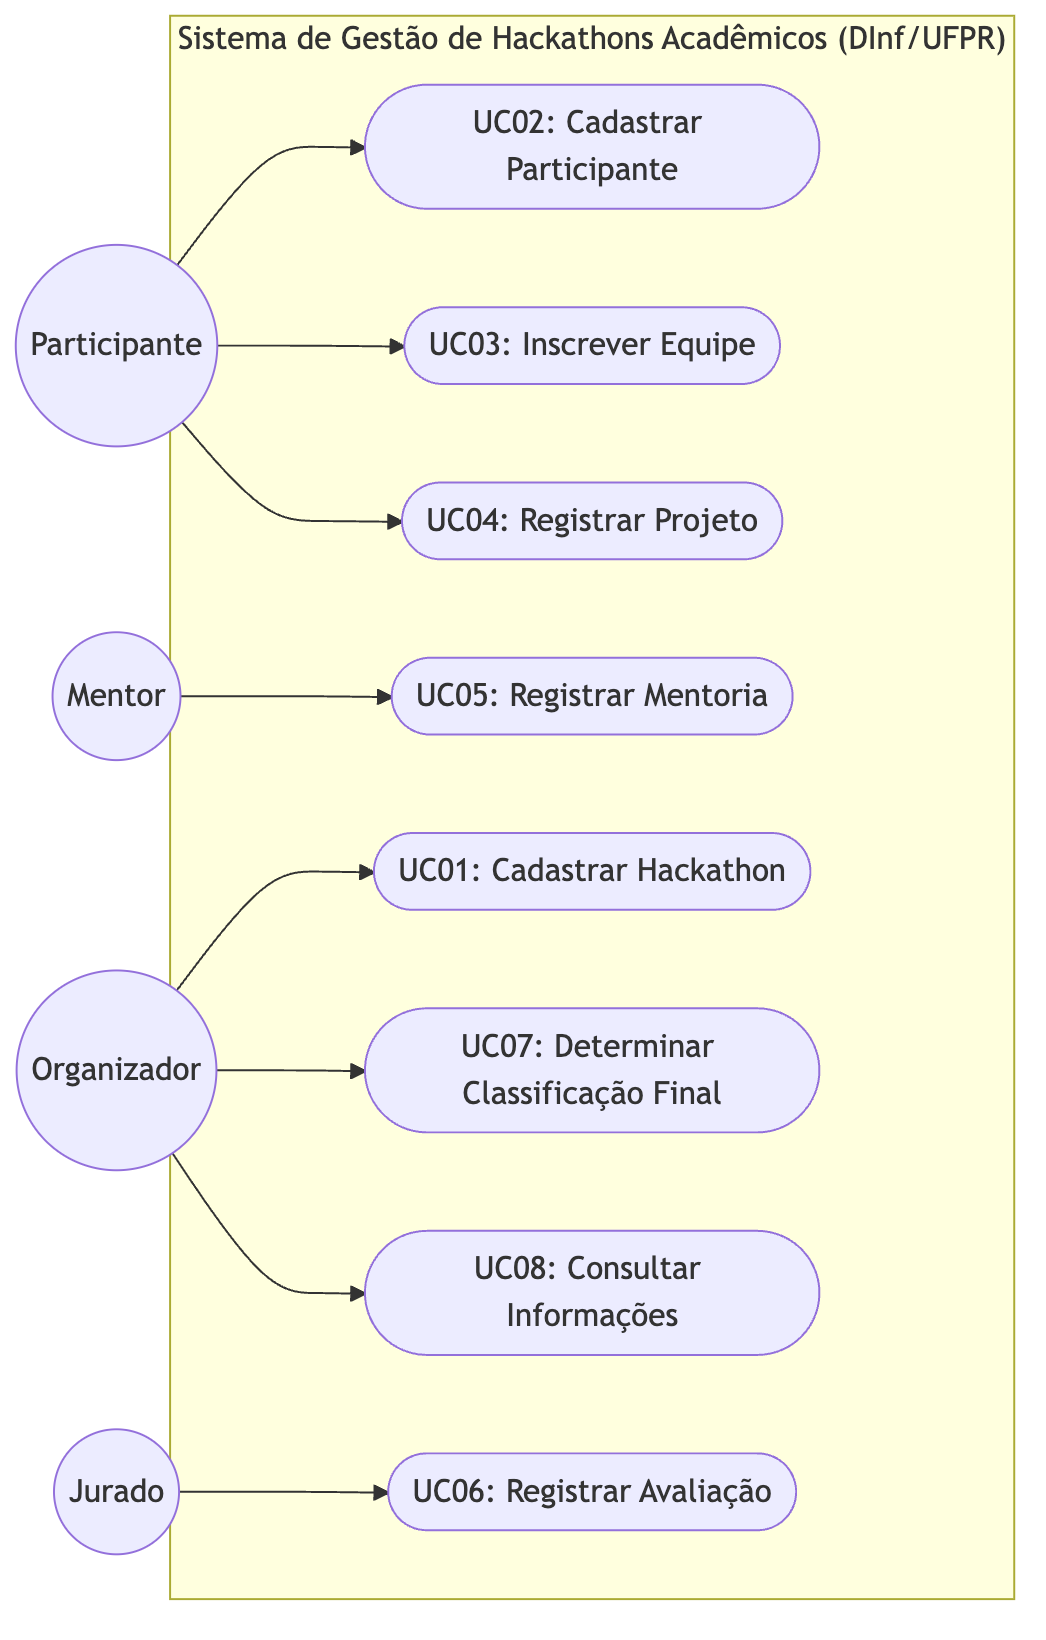
\includegraphics[width=0.95\textwidth]{images/uc_diagram.png}
\caption{Diagrama de Casos de Uso do Sistema de Hackathons}
\label{fig:uc_diagram}
\end{figure}

A seguir, são apresentadas as especificações detalhadas dos casos de uso centrais no padrão da disciplina.

\subsection{ECU 001: Cadastrar Hackathon}
\begin{table}[H]
\centering
\small
\begin{tabular}{|p{3.2cm}|p{11.5cm}|}
\hline
\textbf{Nome} & Cadastrar Hackathon \\ \hline
\textbf{Descrição} & Permite ao organizador criar uma nova edição de Hackathon no sistema. \\ \hline
\textbf{Atores} & Organizador. \\ \hline
\textbf{Fluxo Básico} & 
1. O Organizador acessa a opção de cadastrar hackathon. \newline
2. O sistema exibe o formulário com: Nome, Data de Início, Data de Término, Número Máximo de Equipes e Descrição. \newline
3. O Organizador preenche os dados e confirma o cadastro. \newline
4. O sistema valida os campos, persiste o novo hackathon e exibe mensagem de sucesso. \\ \hline
\textbf{Fluxos Alternativos} & 
A. Caso a data de término seja anterior à data de início ou o número de equipes seja menor que 1, o sistema exibe mensagem de erro e solicita correção. \\ \hline
\textbf{Pré-condições} & O Organizador deve estar na interface de administração. \\ \hline
\textbf{Pós-condições} & Uma nova instância de Hackathon é criada e salva no banco de dados. \\ \hline
\end{tabular}
\end{table}

\subsection{ECU 002: Cadastrar Participante}
\begin{table}[H]
\centering
\small
\begin{tabular}{|p{3.2cm}|p{11.5cm}|}
\hline
\textbf{Nome} & Cadastrar Participante \\ \hline
\textbf{Descrição} & Registra um novo estudante como participante apto a integrar equipes. \\ \hline
\textbf{Atores} & Participante / Estudante. \\ \hline
\textbf{Fluxo Básico} & 
1. O estudante acessa a tela de cadastro de participante. \newline
2. O sistema solicita: Nome Completo, E-mail Institucional, Curso e GRR/Matrícula. \newline
3. O estudante preenche os campos e confirma o envio. \newline
4. O sistema valida a unicidade do GRR/e-mail, cadastra o participante e confirma a operação. \\ \hline
\textbf{Fluxos Alternativos} & 
A. Se o GRR ou e-mail já estiverem cadastrados, o sistema alerta a duplicidade e cancela a operação. \\ \hline
\textbf{Pré-condições} & O estudante possui vínculo ativo com a universidade. \\ \hline
\textbf{Pós-condições} & O participante passa a constar na lista de estudantes disponíveis. \\ \hline
\end{tabular}
\end{table}

\subsection{ECU 003: Inscrever Equipe}
\begin{table}[H]
\centering
\small
\begin{tabular}{|p{3.2cm}|p{11.5cm}|}
\hline
\textbf{Nome} & Inscrever Equipe \\ \hline
\textbf{Descrição} & Inscreve uma nova equipe em um Hackathon específico com seus integrantes. \\ \hline
\textbf{Atores} & Participante (Líder da Equipe). \\ \hline
\textbf{Fluxo Básico} & 
1. O participante seleciona o Hackathon e acessa a inscrição de equipe. \newline
2. O sistema exibe o formulário com Nome da Equipe e seleção dos Participantes. \newline
3. O participante informa o nome da equipe e seleciona 1 ou mais membros. \newline
4. O sistema verifica a capacidade do evento e a elegibilidade dos membros. \newline
5. O sistema registra a equipe, associa os membros ao evento e exibe confirmação. \\ \hline
\textbf{Fluxos Alternativos} & 
A. Se o Hackathon tiver atingido o limite ($maxEquipes$), o sistema rejeita a inscrição informando lotação. \newline
B. Se algum participante já pertencer a outra equipe no mesmo hackathon, o sistema notifica o conflito. \\ \hline
\textbf{Pré-condições} & Hackathon criado e participantes previamente cadastrados. \\ \hline
\textbf{Pós-condições} & Uma nova Equipe é instanciada e vinculada ao Hackathon e aos seus membros. \\ \hline
\end{tabular}
\end{table}

\subsection{ECU 004: Registrar Projeto}
\begin{table}[H]
\centering
\small
\begin{tabular}{|p{3.2cm}|p{11.5cm}|}
\hline
\textbf{Nome} & Registrar Projeto \\ \hline
\textbf{Descrição} & Registra o projeto desenvolvido pela equipe durante o hackathon. \\ \hline
\textbf{Atores} & Participante (Membro da Equipe). \\ \hline
\textbf{Fluxo Básico} & 
1. O membro da equipe seleciona sua equipe e acessa o cadastro de projeto. \newline
2. O sistema exibe os campos: Título, Descrição do Projeto e Área Temática. \newline
3. O participante preenche as informações e confirma o registro. \newline
4. O sistema valida que a equipe ainda não possui projeto e salva o registro. \\ \hline
\textbf{Fluxos Alternativos} & 
A. Caso a equipe já possua um projeto cadastrado no evento, o sistema rejeita a operação com mensagem de erro. \\ \hline
\textbf{Pré-condições} & A equipe deve estar devidamente inscrita no Hackathon. \\ \hline
\textbf{Pós-condições} & Exatamente um Projeto é associado à Equipe. \\ \hline
\end{tabular}
\end{table}

\subsection{ECU 005: Registrar Mentoria}
\begin{table}[H]
\centering
\small
\begin{tabular}{|p{3.2cm}|p{11.5cm}|}
\hline
\textbf{Nome} & Registrar Mentoria \\ \hline
\textbf{Descrição} & Permite ao mentor registrar uma sessão de orientação prestada a uma equipe. \\ \hline
\textbf{Atores} & Mentor. \\ \hline
\textbf{Fluxo Básico} & 
1. O Mentor seleciona seu perfil e a equipe atendida. \newline
2. O sistema apresenta o campo para anotações/comentários e registro da data/hora. \newline
3. O Mentor insere as observações técnicas e confirma o registro. \newline
4. O sistema persiste a mentoria e confirma a operação. \\ \hline
\textbf{Fluxos Alternativos} & 
A. Se os comentários estiverem vazios ou os identificadores forem inválidos, o sistema exibe alerta. \\ \hline
\textbf{Pré-condições} & Mentor cadastrado e equipe inscrita no evento. \\ \hline
\textbf{Pós-condições} & Um registro de Mentoria é vinculado ao Mentor e à Equipe atendida. \\ \hline
\end{tabular}
\end{table}

\subsection{ECU 006: Registrar Avaliação}
\begin{table}[H]
\centering
\small
\begin{tabular}{|p{3.2cm}|p{11.5cm}|}
\hline
\textbf{Nome} & Registrar Avaliação \\ \hline
\textbf{Descrição} & Permite ao jurado avaliar o projeto de uma equipe com nota e parecer. \\ \hline
\textbf{Atores} & Jurado. \\ \hline
\textbf{Fluxo Básico} & 
1. O Jurado escolhe o projeto a ser avaliado. \newline
2. O sistema exibe o formulário de avaliação com campo de Nota (0.0 a 10.0) e Comentários/Parecer. \newline
3. O Jurado insere a nota, redige o feedback e confirma o envio. \newline
4. O sistema valida se a nota está no intervalo $[0.0, 10.0]$ e salva a avaliação. \\ \hline
\textbf{Fluxos Alternativos} & 
A. Caso a nota seja menor que 0.0 ou maior que 10.0, o sistema impede o registro e avisa o jurado. \\ \hline
\textbf{Pré-condições} & Jurado cadastrado e projeto registrado pela equipe. \\ \hline
\textbf{Pós-condições} & A Avaliação é criada e associada ao Projeto e ao Jurado. \\ \hline
\end{tabular}
\end{table}

\subsection{ECU 007: Determinar Classificação Final}
\begin{table}[H]
\centering
\small
\begin{tabular}{|p{3.2cm}|p{11.5cm}|}
\hline
\textbf{Nome} & Determinar Classificação Final \\ \hline
\textbf{Descrição} & Computa as notas médias dos projetos e gera o ranking final ordenado do Hackathon. \\ \hline
\textbf{Atores} & Organizador / Público Geral. \\ \hline
\textbf{Fluxo Básico} & 
1. O usuário solicita a visualização do ranking final do Hackathon. \newline
2. O sistema recupera todas as equipes e projetos do evento. \newline
3. Para cada projeto, calcula a média aritmética das notas dos jurados. \newline
4. O sistema ordena os projetos de forma decrescente pela nota média e número de avaliações. \newline
5. Exibe a tabela de classificação e o pódio dos 3 primeiros colocados. \\ \hline
\textbf{Fluxos Alternativos} & 
A. Caso nenhum projeto tenha sido avaliado, o sistema exibe os projetos sem nota calculada. \\ \hline
\textbf{Pré-condições} & Hackathon com equipes e projetos registrados. \\ \hline
\textbf{Pós-condições} & O ranking oficial é gerado e disponibilizado para consulta. \\ \hline
\end{tabular}
\end{table}

\section{Modelo Conceitual de Domínio}

O Modelo Conceitual de Domínio captura os conceitos do mundo real e seus relacionamentos estruturais no contexto dos Hackathons do DInf/UFPR, conforme ilustrado na Figura~\ref{fig:domain_model}.

\begin{figure}[H]
\centering
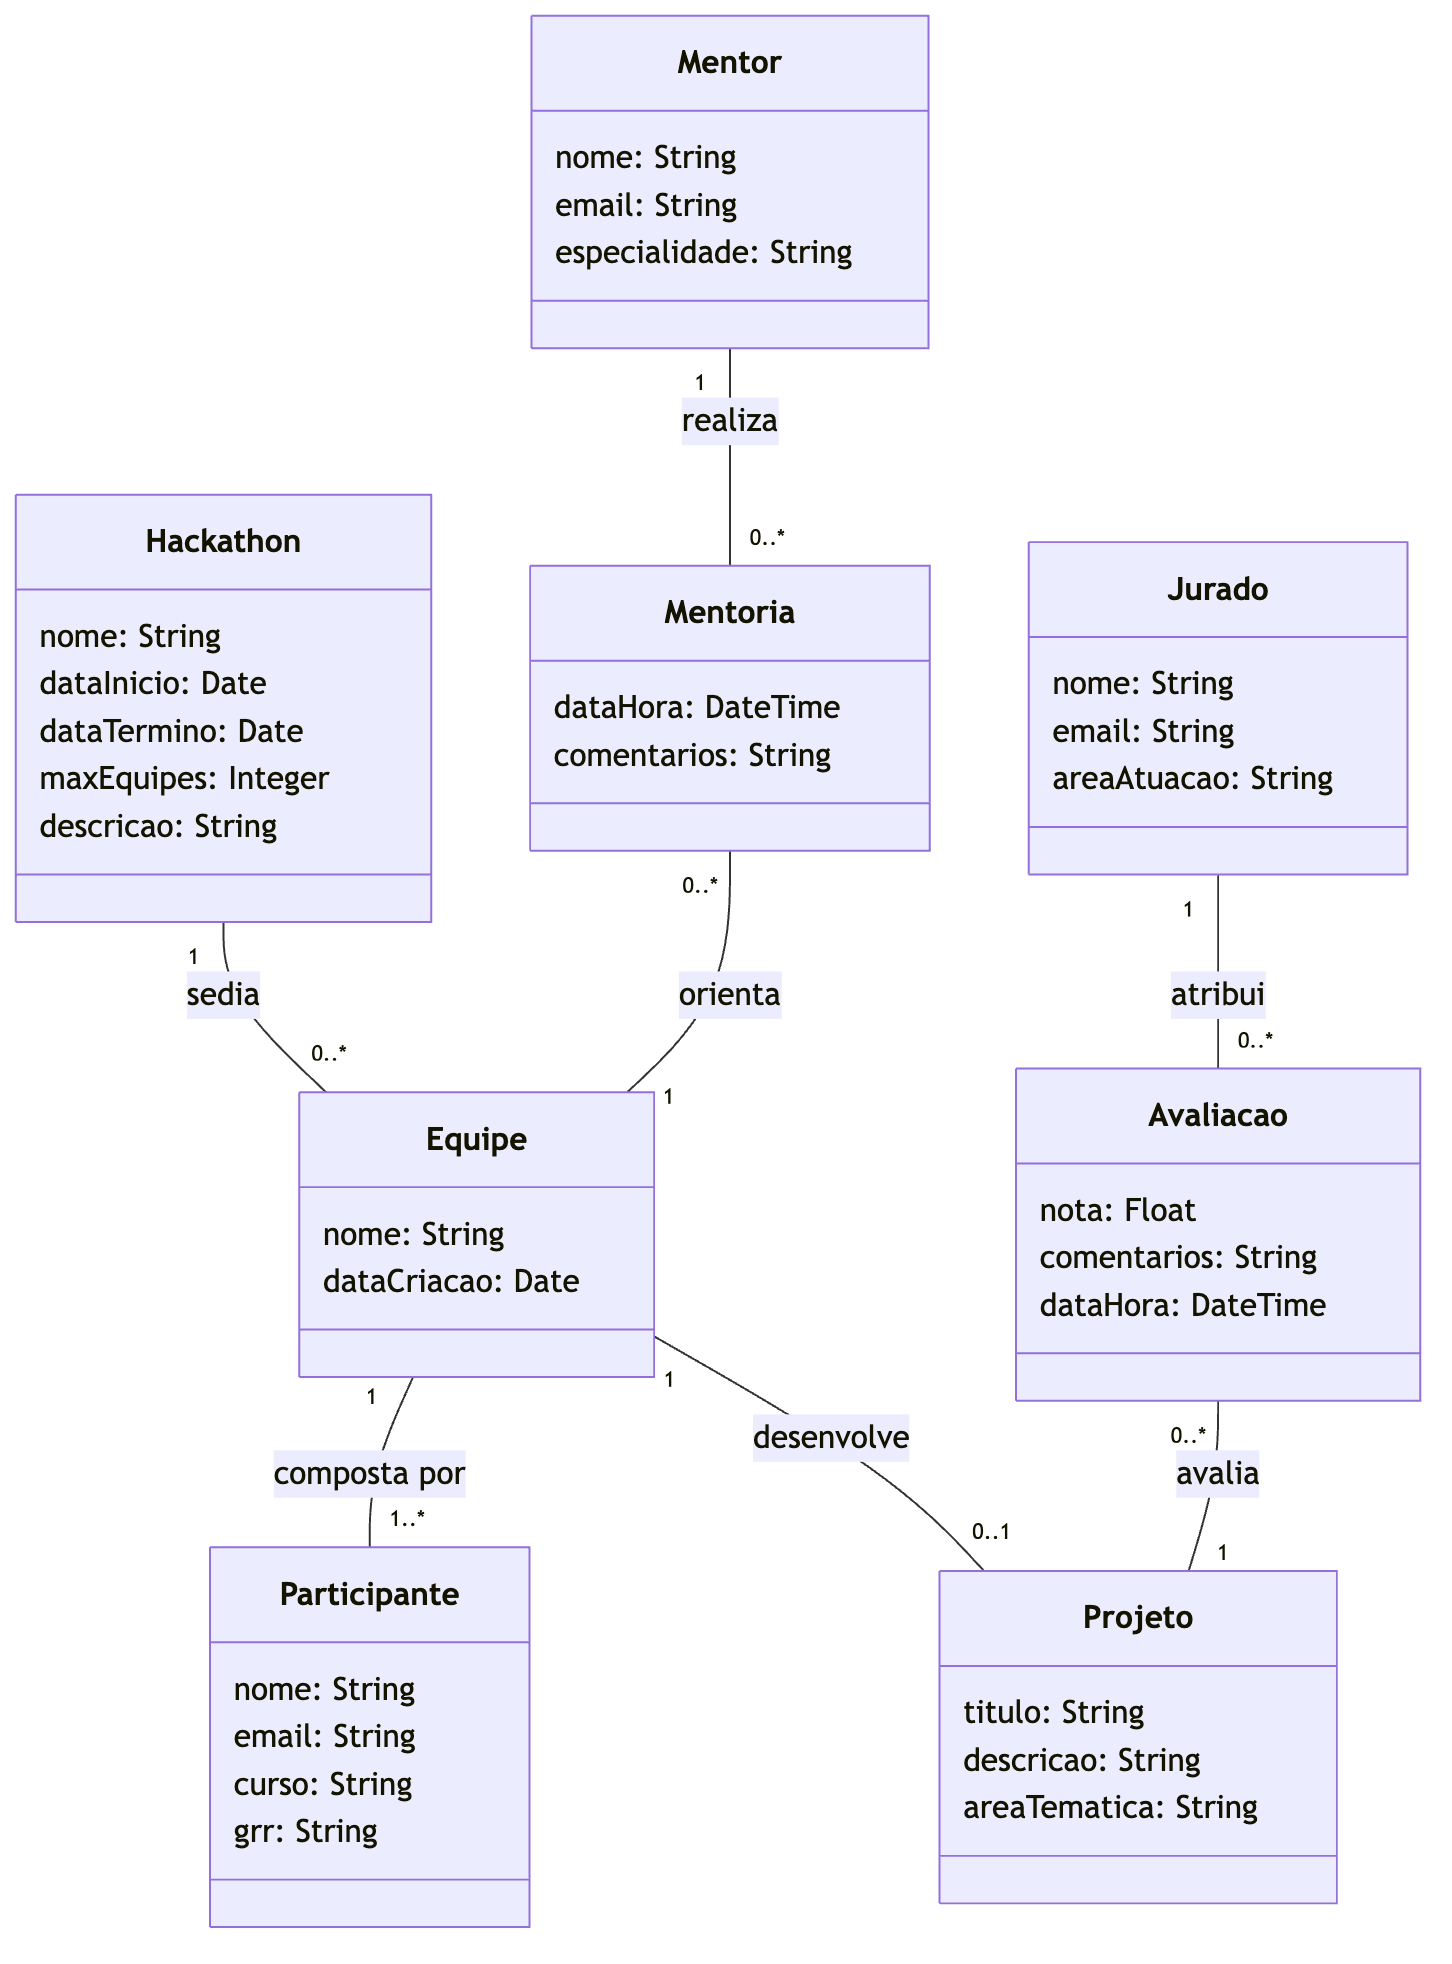
\includegraphics[width=0.92\textwidth]{images/domain_model.png}
\caption{Modelo Conceitual de Domínio (Classes Conceituais)}
\label{fig:domain_model}
\end{figure}

As principais associações e multiplicidades conceituais estabelecidas são:
\begin{itemize}
    \item Um \texttt{Hackathon} agrega de 0 a $N$ instâncias de \texttt{Equipe}.
    \item Cada \texttt{Equipe} é composta por 1 a $N$ instâncias de \texttt{Participante}.
    \item Cada \texttt{Equipe} desenvolve no máximo 1 \texttt{Projeto} ($0..1$).
    \item Um \texttt{Mentor} realiza 0 a $N$ \texttt{Mentorias}, e cada \texttt{Mentoria} orienta 1 \texttt{Equipe}.
    \item Um \texttt{Jurado} atribui 0 a $N$ \texttt{Avaliações}, e cada \texttt{Avaliação} examina 1 \texttt{Projeto}.
\end{itemize}

\section{Diagramas de Sequência de Sistema (DSS)}

Os Diagramas de Sequência de Sistema (DSS) descrevem o comportamento de caixa-preta do sistema, capturando os eventos de entrada gerados pelos atores externos para a fronteira do \texttt{:Sistema}.

\begin{figure}[H]
\centering
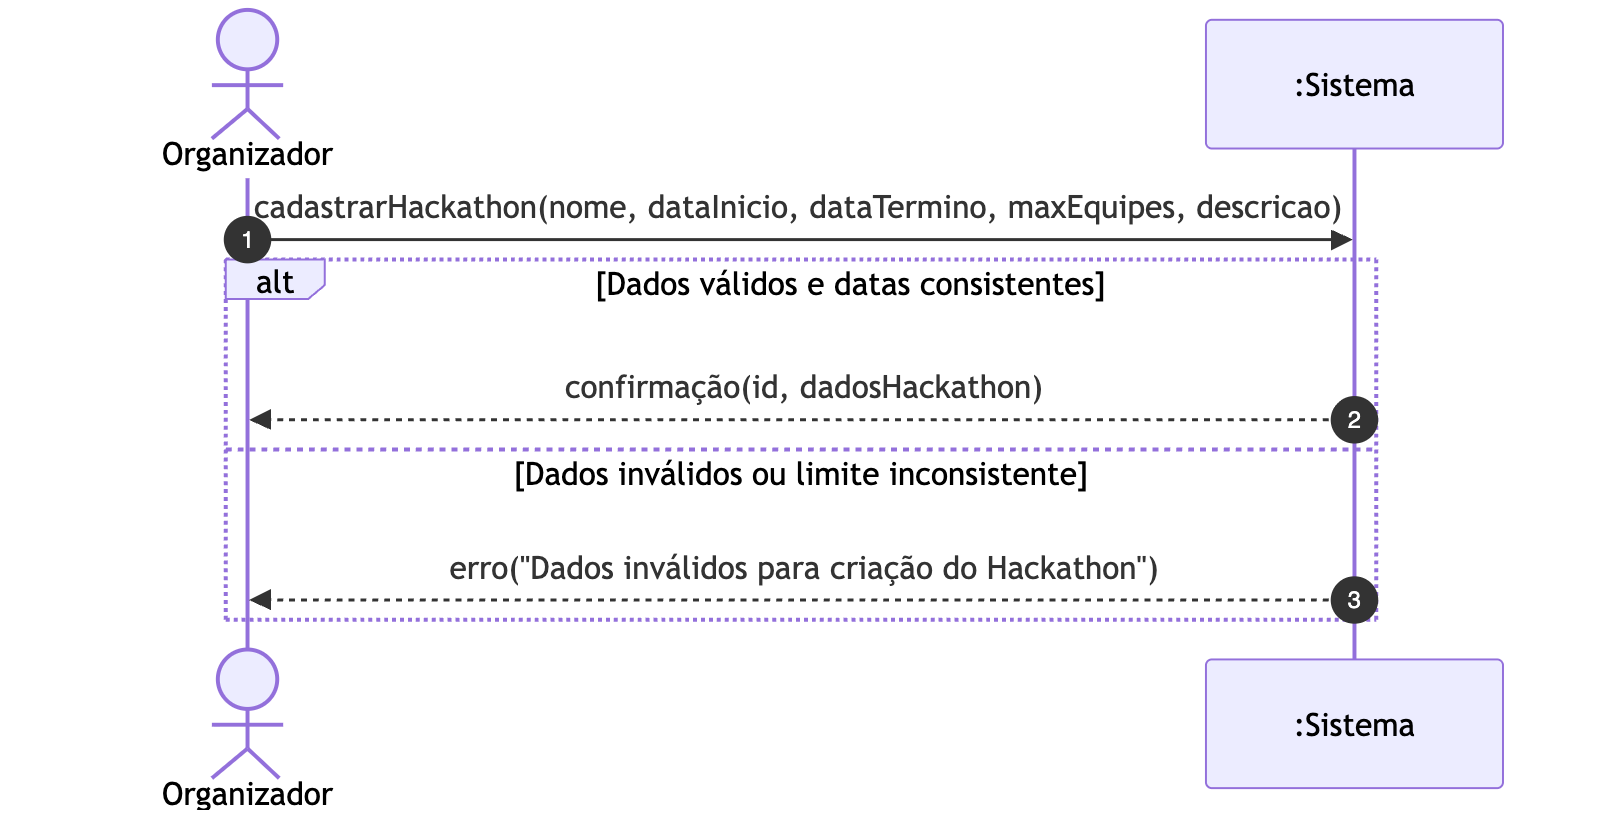
\includegraphics[width=0.85\textwidth]{images/dss_001_cadastrar_hackathon.png}
\caption{DSS 001: Cadastrar Hackathon}
\label{fig:dss001}
\end{figure}

\begin{figure}[H]
\centering
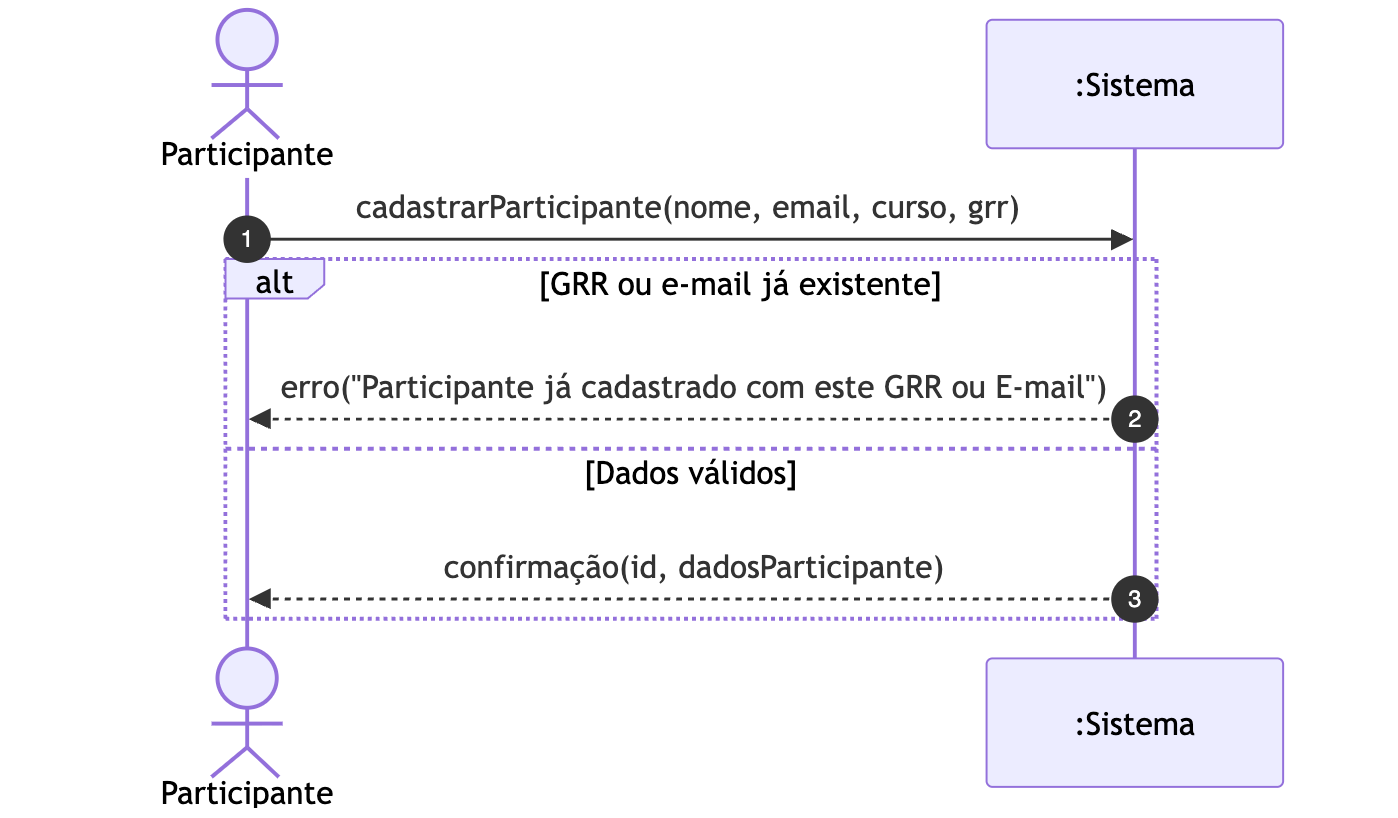
\includegraphics[width=0.85\textwidth]{images/dss_002_cadastrar_participante.png}
\caption{DSS 002: Cadastrar Participante}
\label{fig:dss002}
\end{figure}

\begin{figure}[H]
\centering
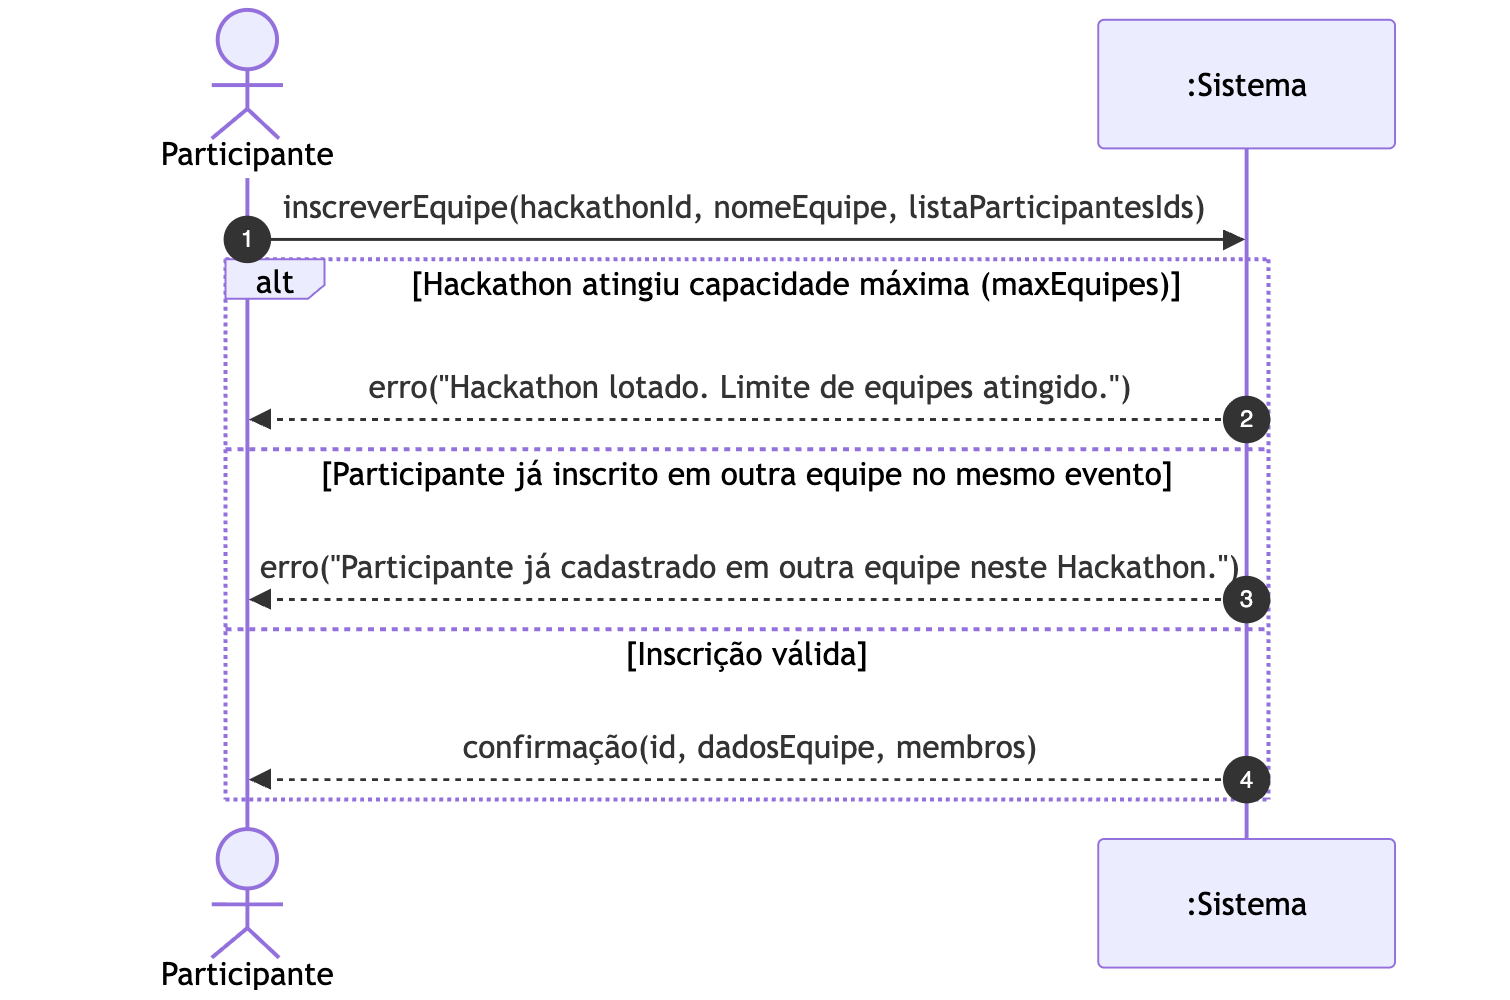
\includegraphics[width=0.85\textwidth]{images/dss_003_inscrever_equipe.png}
\caption{DSS 003: Inscrever Equipe}
\label{fig:dss003}
\end{figure}

\begin{figure}[H]
\centering
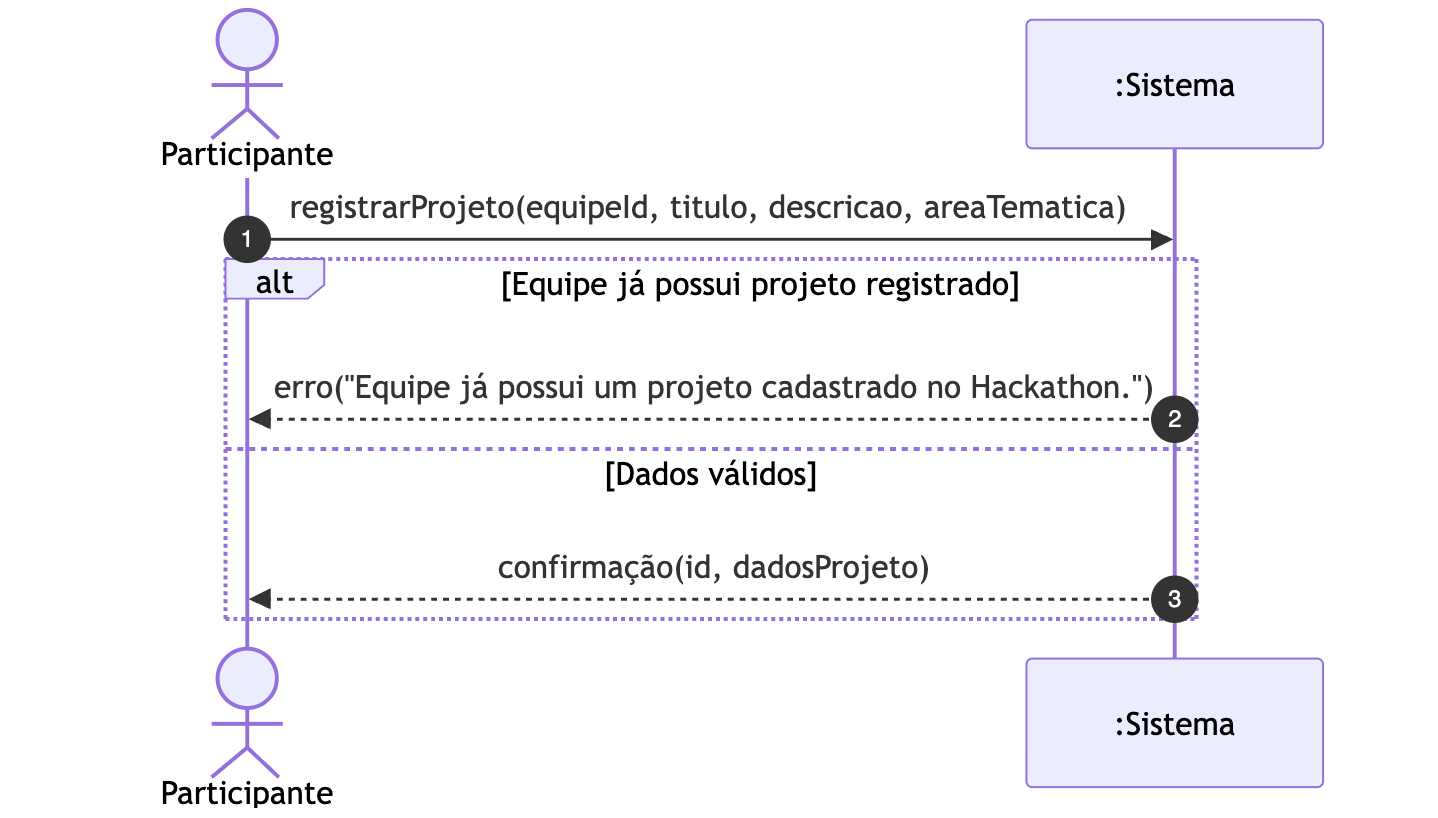
\includegraphics[width=0.85\textwidth]{images/dss_004_registrar_projeto.png}
\caption{DSS 004: Registrar Projeto}
\label{fig:dss004}
\end{figure}

\begin{figure}[H]
\centering
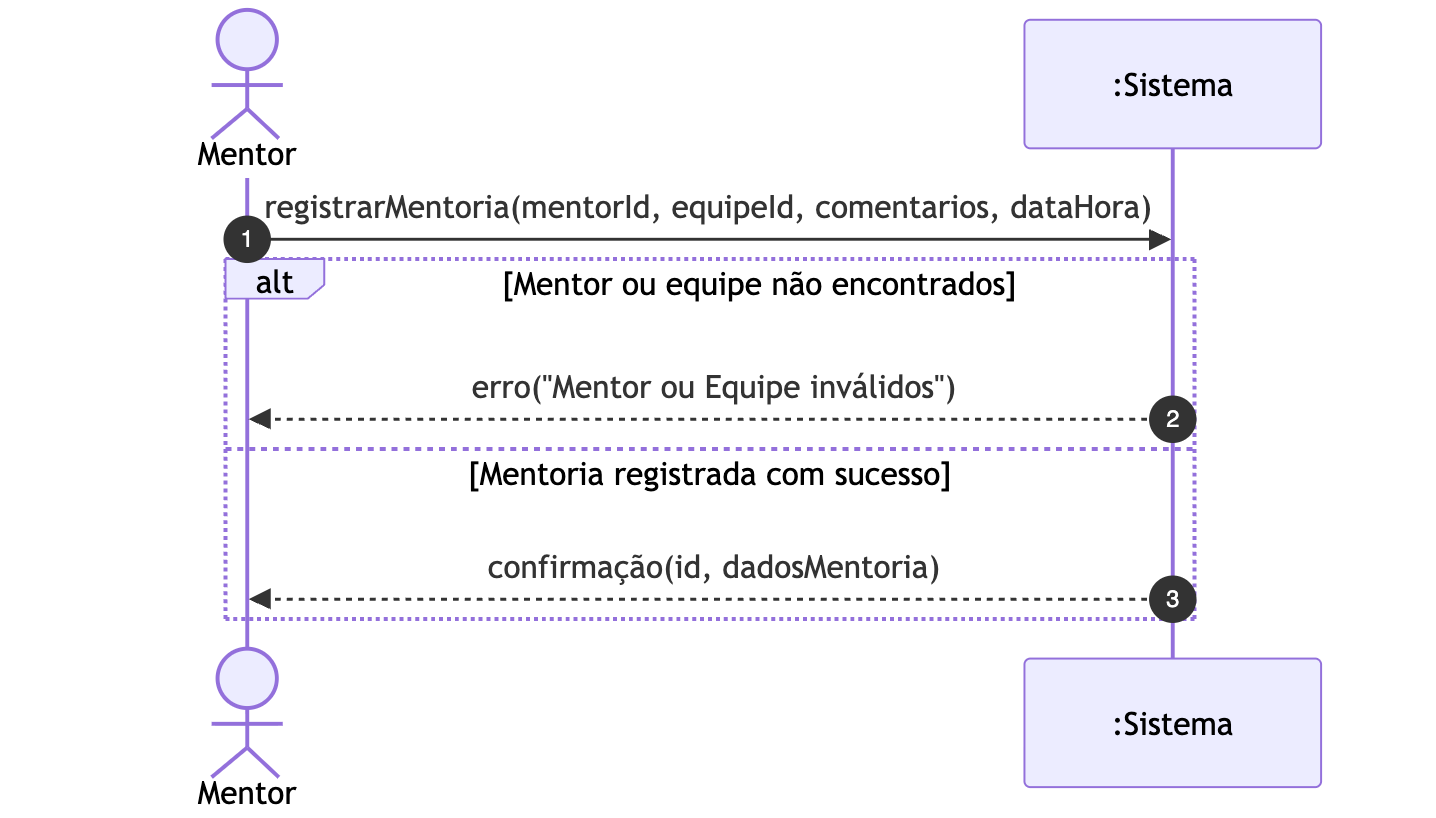
\includegraphics[width=0.85\textwidth]{images/dss_005_registrar_mentoria.png}
\caption{DSS 005: Registrar Mentoria}
\label{fig:dss005}
\end{figure}

\begin{figure}[H]
\centering
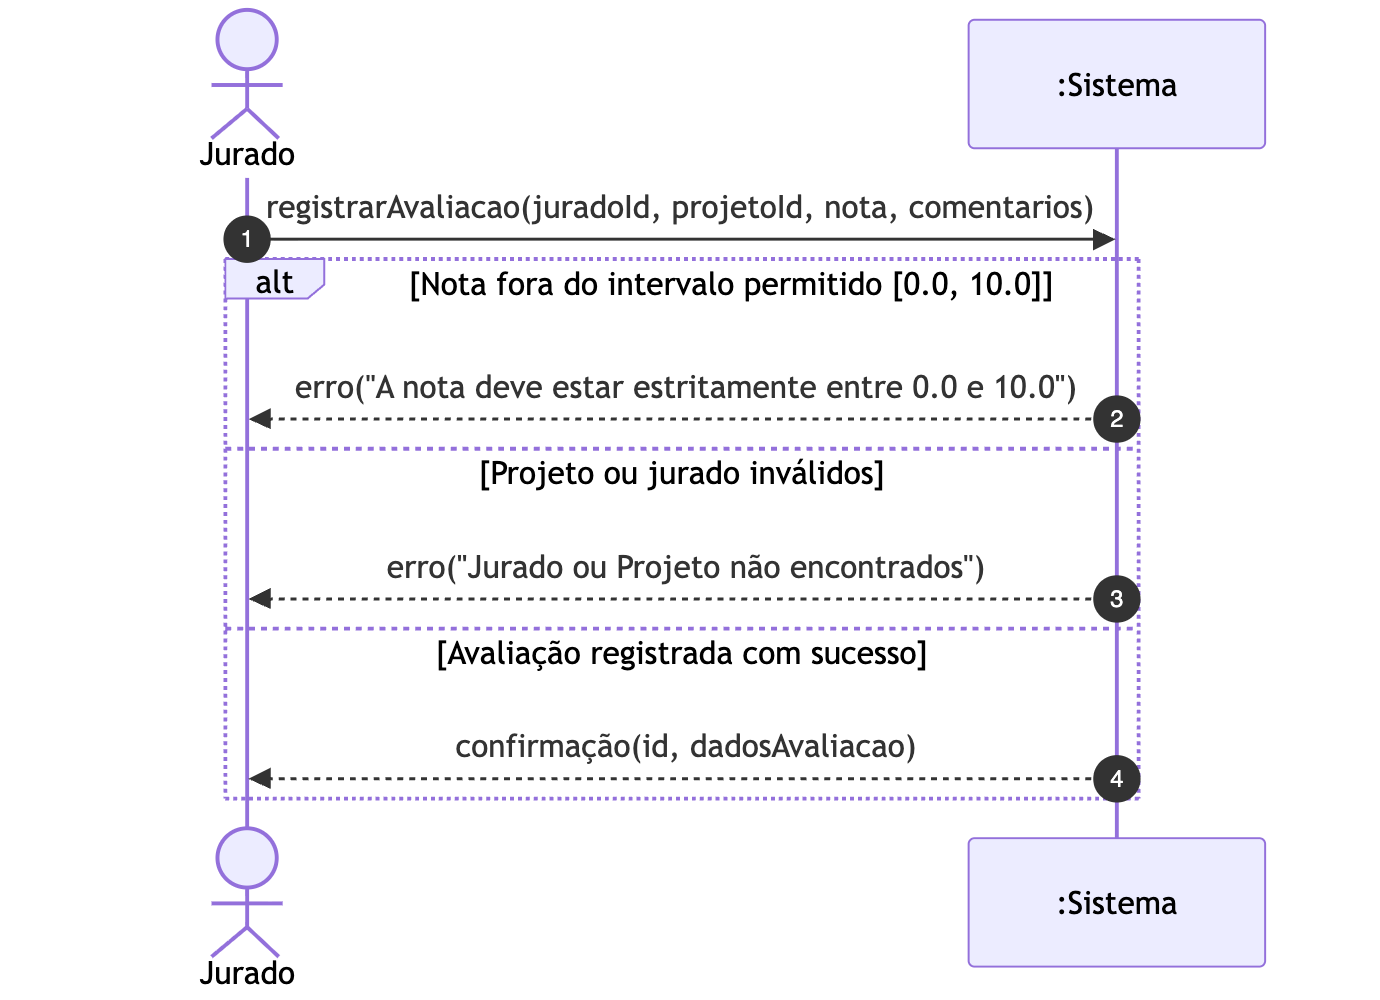
\includegraphics[width=0.85\textwidth]{images/dss_006_registrar_avaliacao.png}
\caption{DSS 006: Registrar Avaliação}
\label{fig:dss006}
\end{figure}

\begin{figure}[H]
\centering
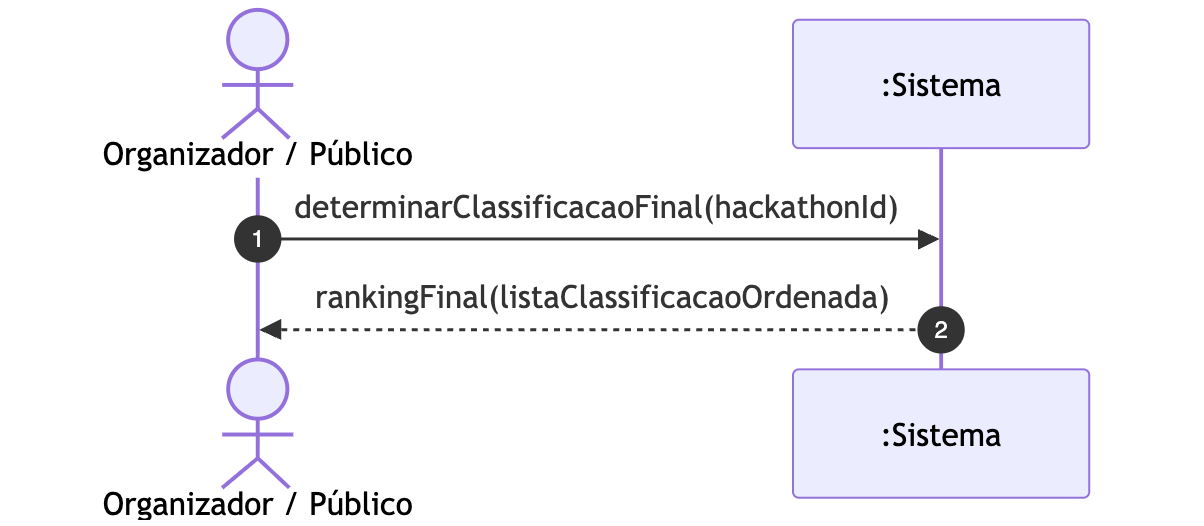
\includegraphics[width=0.85\textwidth]{images/dss_007_calcular_ranking.png}
\caption{DSS 007: Determinar Classificação Final}
\label{fig:dss007}
\end{figure}

\section{Contratos de Operação (Padrão Craig Larman)}

Para cada operação de sistema identificada nos DSS, elaboramos os Contratos de Operação formais especificando rigorosamente as pré-condições e as transformações de estado nas pós-condições.

\subsection{Contrato 01: cadastrarHackathon}
\begin{itemize}
    \item \textbf{Operação}: \texttt{cadastrarHackathon(nome: String, dataInicio: Date, dataTermino: Date, maxEquipes: Integer, descricao: String)}
    \item \textbf{Referências Cruzadas}: ECU 001 (Cadastrar Hackathon).
    \item \textbf{Pré-condições}: \texttt{nome} não nulo; \texttt{dataTermino} $\ge$ \texttt{dataInicio}; \texttt{maxEquipes} $\ge 1$.
    \item \textbf{Pós-condições}:
    \begin{itemize}
        \item Uma instância $h$ de \texttt{Hackathon} foi criada.
        \item Os atributos de $h$ foram inicializados com os parâmetros fornecidos.
        \item A instância $h$ foi registrada no repositório de hackathons.
    \end{itemize}
\end{itemize}

\subsection{Contrato 02: cadastrarParticipante}
\begin{itemize}
    \item \textbf{Operação}: \texttt{cadastrarParticipante(nome: String, email: String, curso: String, grr: String)}
    \item \textbf{Referências Cruzadas}: ECU 002 (Cadastrar Participante).
    \item \textbf{Pré-condições}: \texttt{email} e \texttt{grr} não registrados previamente.
    \item \textbf{Pós-condições}:
    \begin{itemize}
        \item Uma instância $p$ de \texttt{Participante} foi criada.
        \item Os atributos de $p$ foram atribuídos.
        \item A instância $p$ foi persistida no repositório de participantes.
    \end{itemize}
\end{itemize}

\subsection{Contrato 03: inscreverEquipe}
\begin{itemize}
    \item \textbf{Operação}: \texttt{inscreverEquipe(hackathonId: Integer, nome: String, participanteIds: List<Integer>)}
    \item \textbf{Referências Cruzadas}: ECU 003 (Inscrever Equipe).
    \item \textbf{Pré-condições}:
    \begin{itemize}
        \item O Hackathon com \texttt{hackathonId} existe e o total de equipes inscritas é menor que \texttt{maxEquipes}.
        \item Todos os \texttt{participanteIds} existem e nenhum deles pertence a outra equipe no mesmo hackathon.
    \end{itemize}
    \item \textbf{Pós-condições}:
    \begin{itemize}
        \item Uma instância $e$ de \texttt{Equipe} foi criada.
        \item Uma associação foi formada entre $h$ (\texttt{Hackathon}) e $e$.
        \item Associações foram formadas entre $e$ e cada participante da lista.
    \end{itemize}
\end{itemize}

\subsection{Contrato 04: registrarProjeto}
\begin{itemize}
    \item \textbf{Operação}: \texttt{registrarProjeto(equipeId: Integer, titulo: String, descricao: String, areaTematica: String)}
    \item \textbf{Referências Cruzadas}: ECU 004 (Registrar Projeto).
    \item \textbf{Pré-condições}: A equipe $e$ existe e não possui nenhum projeto associado previamente.
    \item \textbf{Pós-condições}:
    \begin{itemize}
        \item Uma instância $proj$ de \texttt{Projeto} foi criada.
        \item Uma associação exclusiva foi formada entre a equipe $e$ e o projeto $proj$.
    \end{itemize}
\end{itemize}

\subsection{Contrato 05: registrarMentoria}
\begin{itemize}
    \item \textbf{Operação}: \texttt{registrarMentoria(mentorId: Integer, equipeId: Integer, comentarios: String, dataHora: DateTime)}
    \item \textbf{Referências Cruzadas}: ECU 005 (Registrar Mentoria).
    \item \textbf{Pré-condições}: O mentor $m$ e a equipe $e$ existem no sistema.
    \item \textbf{Pós-condições}:
    \begin{itemize}
        \item Uma instância $men$ de \texttt{Mentoria} foi criada.
        \item Foram formadas associações entre $m$ e $men$, e entre $men$ e $e$.
    \end{itemize}
\end{itemize}

\subsection{Contrato 06: registrarAvaliacao}
\begin{itemize}
    \item \textbf{Operação}: \texttt{registrarAvaliacao(juradoId: Integer, projetoId: Integer, nota: Float, comentarios: String)}
    \item \textbf{Referências Cruzadas}: ECU 006 (Registrar Avaliação).
    \item \textbf{Pré-condições}: O jurado $j$ e o projeto $proj$ existem; $0.0 \le \texttt{nota} \le 10.0$.
    \item \textbf{Pós-condições}:
    \begin{itemize}
        \item Uma instância $av$ de \texttt{Avaliacao} foi criada com os atributos fornecidos.
        \item Foram estabelecidas associações entre $j$ e $av$, e entre $av$ e $proj$.
    \end{itemize}
\end{itemize}

\subsection{Contrato 07: determinarClassificacaoFinal}
\begin{itemize}
    \item \textbf{Operação}: \texttt{determinarClassificacaoFinal(hackathonId: Integer): List<ItemClassificacao>}
    \item \textbf{Referências Cruzadas}: ECU 007 (Determinar Classificação Final).
    \item \textbf{Pré-condições}: O Hackathon com \texttt{hackathonId} existe.
    \item \textbf{Pós-condições}:
    \begin{itemize}
        \item Para cada projeto, a nota média foi calculada a partir de suas avaliações.
        \item Uma lista ordenada decrescentemente por nota média foi gerada contendo os objetos de resultado.
    \end{itemize}
\end{itemize}

\section{Diagramas de Interação e Aplicação de Padrões GRASP}

Na fase de projeto orientado a objetos, atribuímos responsabilidades aos componentes aplicando rigorosamente os princípios e padrões fundamentais do GRASP:

\begin{enumerate}
    \item \textbf{Controller (Controlador)}: Classes controladoras especializadas (\texttt{EquipeController}, \texttt{ProjetoController}, \texttt{AvaliacaoController}, \texttt{ClassificacaoController}) recebem as requisições HTTP da camada de apresentação e orquestram a execução dos casos de uso, sem acoplar a UI às regras de domínio.
    \item \textbf{Information Expert (Especialista na Informação)}: O cálculo da nota média foi atribuído à entidade \texttt{Projeto}, pois ela detém o conhecimento direto sobre as avaliações que lhe foram atribuídas.
    \item \textbf{Creator (Criador)}: Os controladores são responsáveis por instanciar as entidades e delegar a persistência aos seus respectivos repositórios.
    \item \textbf{Low Coupling \& High Cohesion (Baixo Acoplamento e Alta Coesão)}: O sistema adota isolamento estrito entre apresentação, aplicação, domínio e infraestrutura de banco de dados.
\end{enumerate}

As Figuras~\ref{fig:sd_inscrever_equipe}, \ref{fig:sd_registrar_projeto}, \ref{fig:sd_registrar_avaliacao} e \ref{fig:sd_calcular_ranking} exibem os Diagramas de Sequência de Projeto.

\begin{figure}[H]
\centering
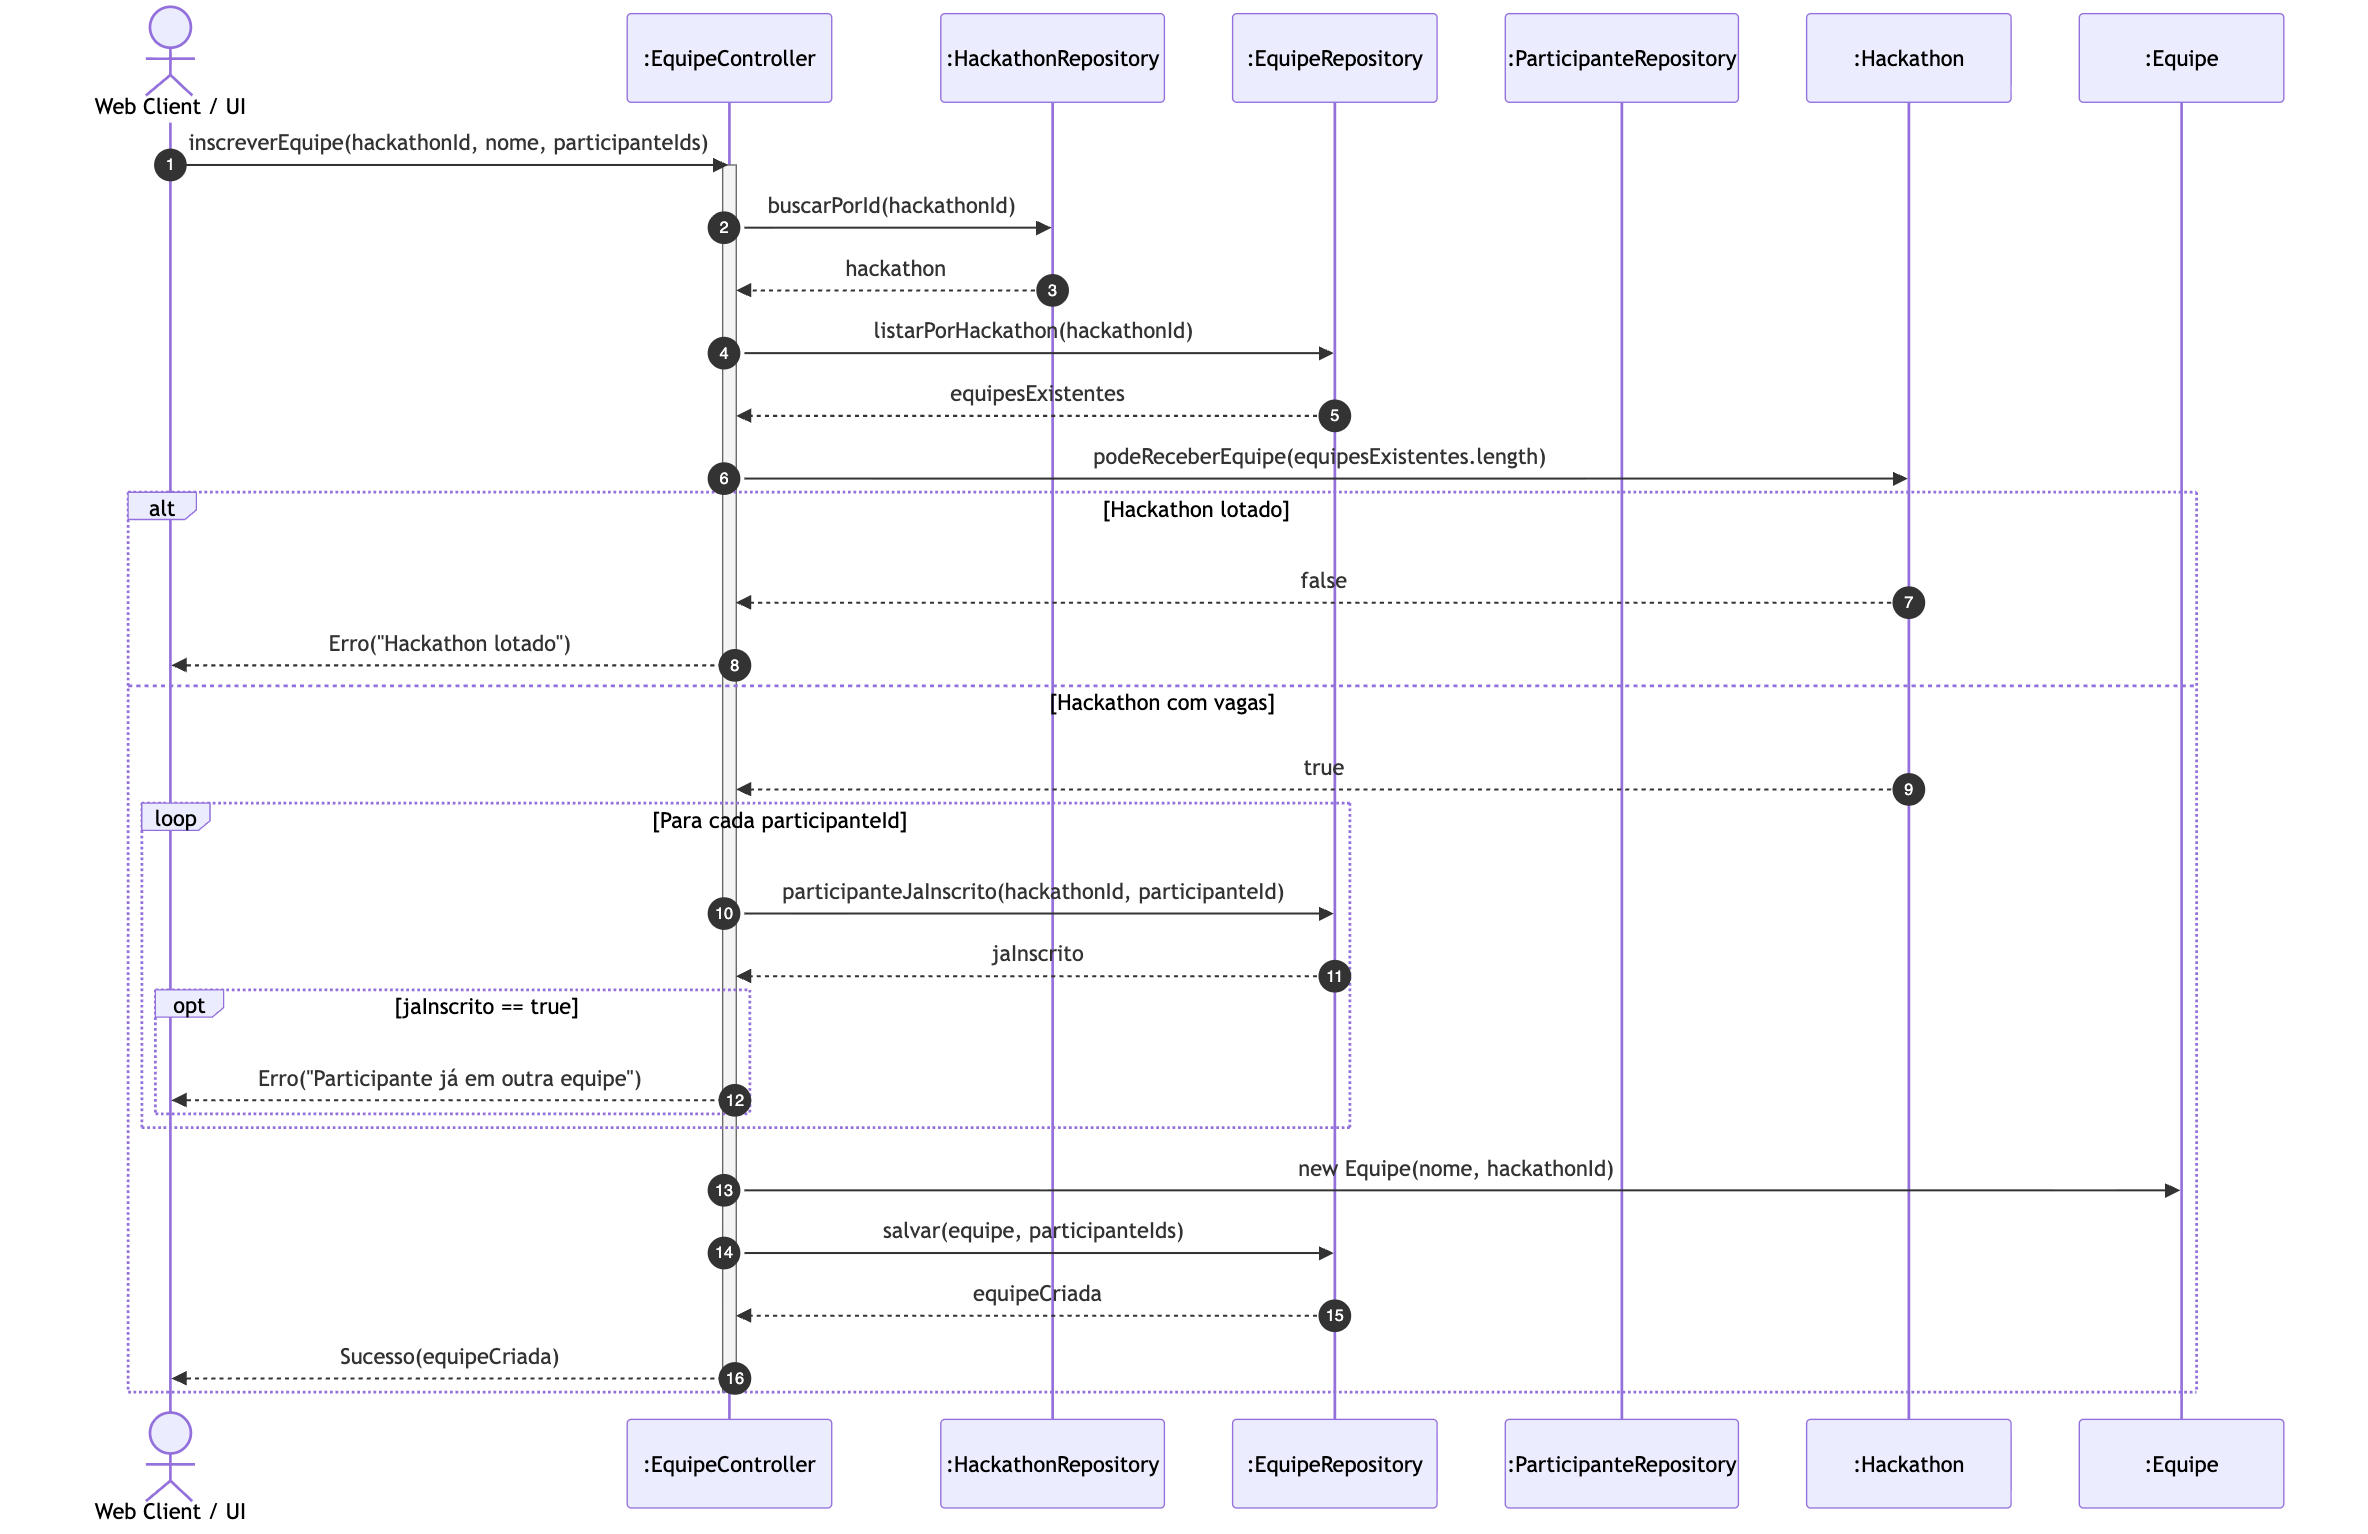
\includegraphics[width=0.92\textwidth]{images/sd_inscrever_equipe.png}
\caption{Diagrama de Sequência de Projeto: Inscrever Equipe}
\label{fig:sd_inscrever_equipe}
\end{figure}

\begin{figure}[H]
\centering
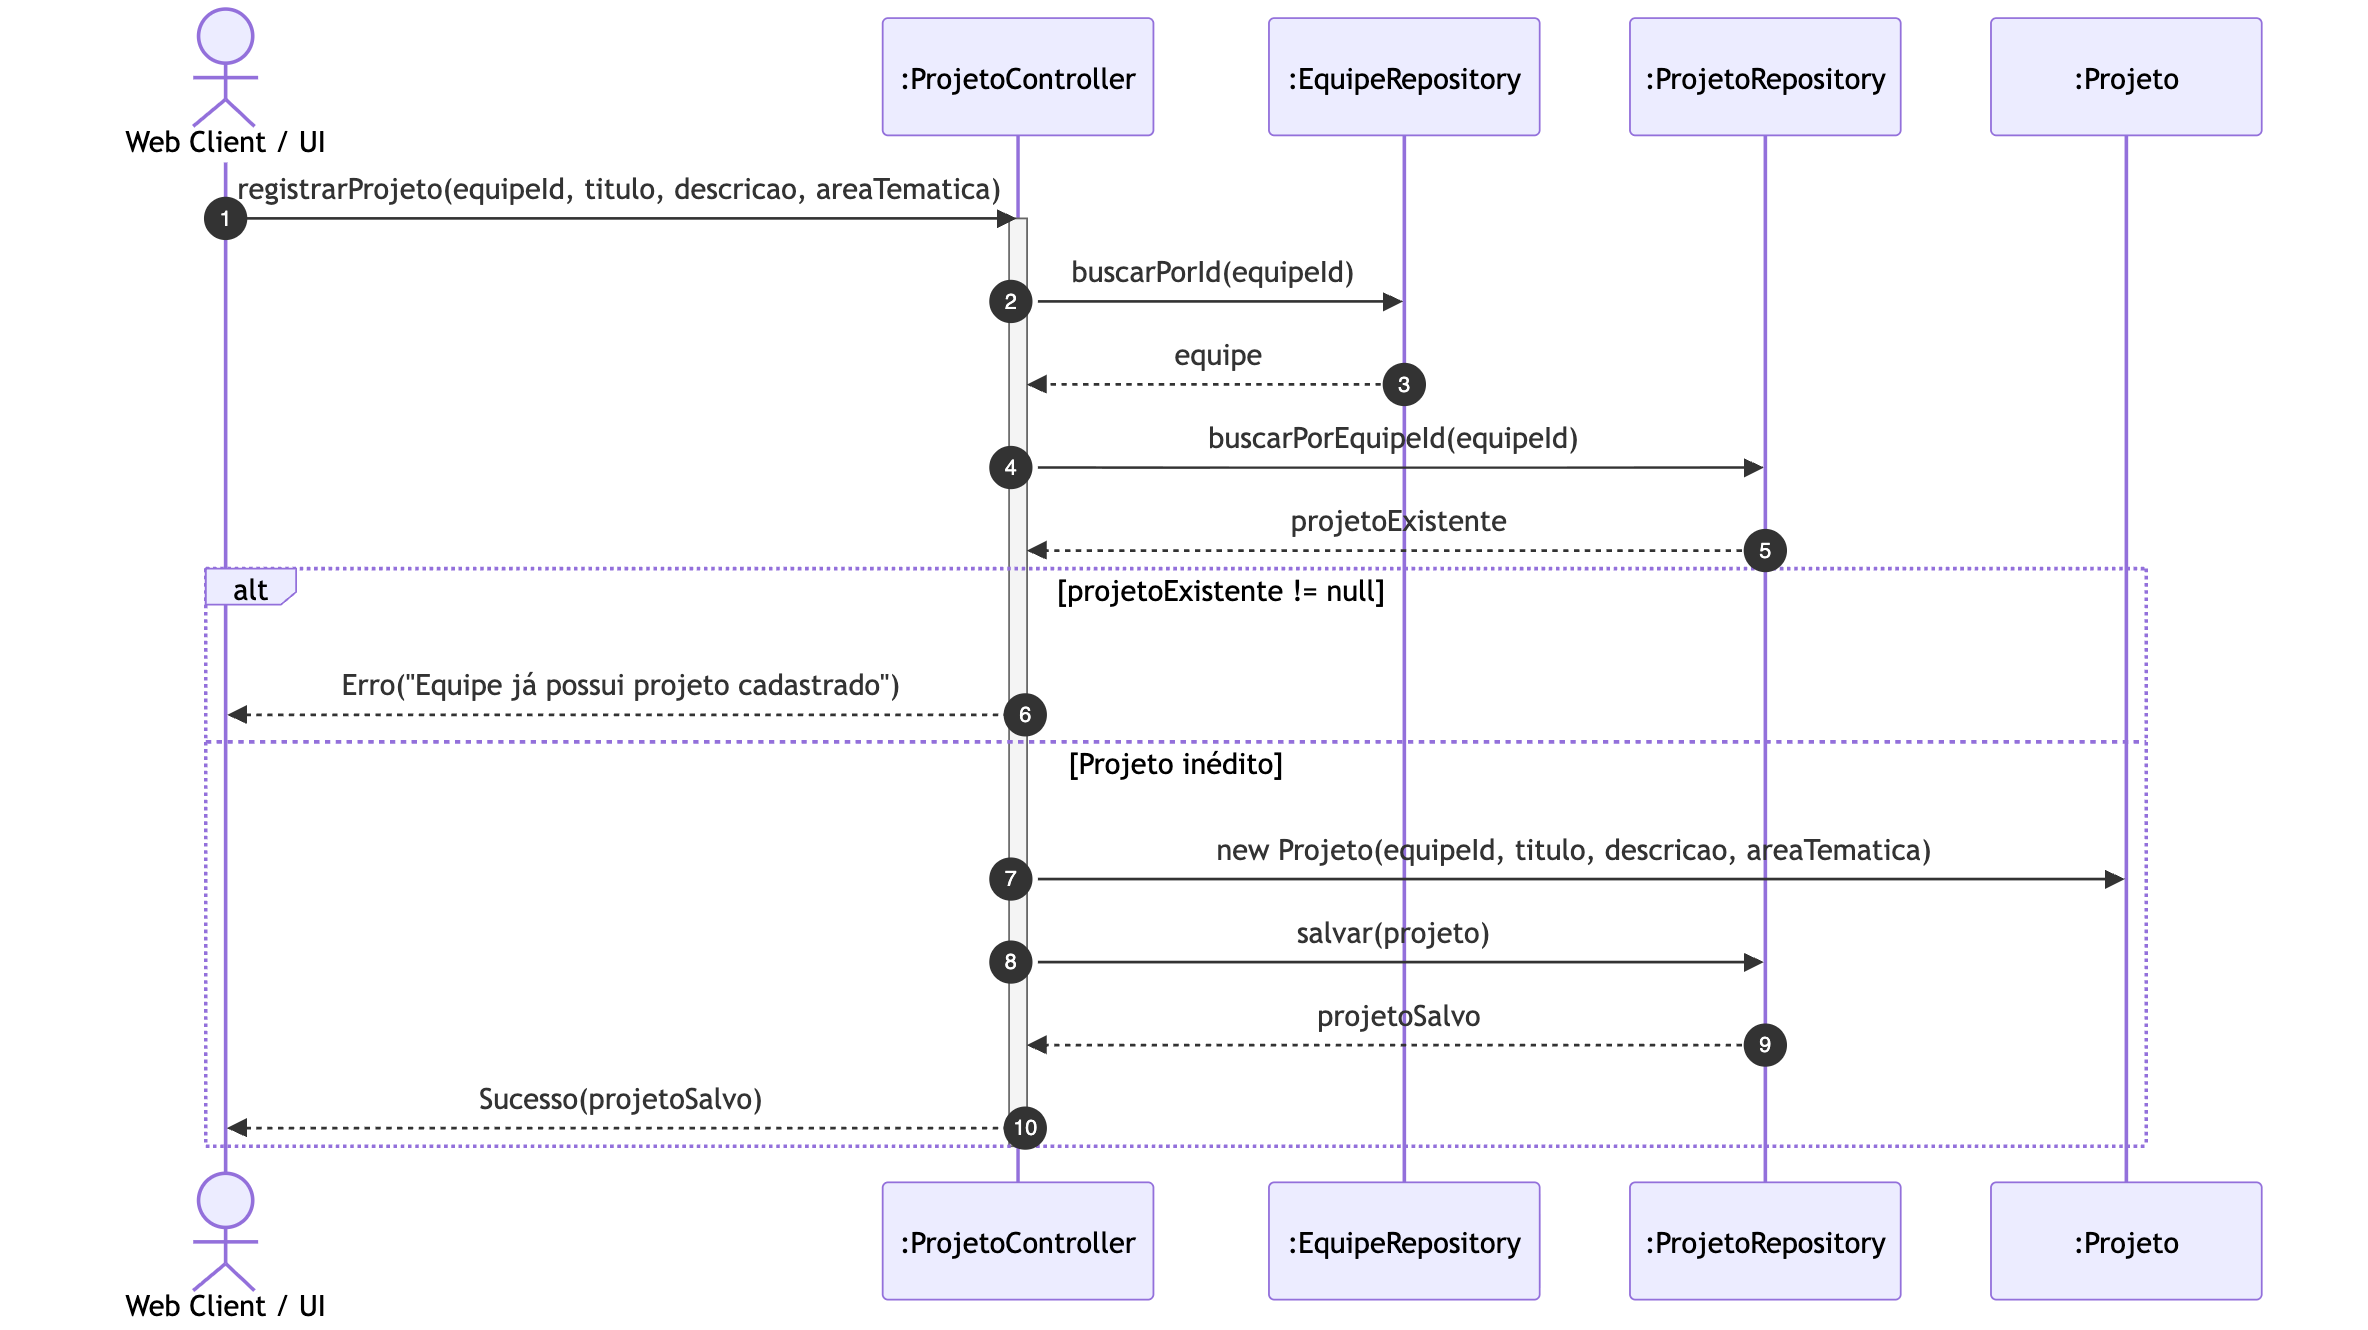
\includegraphics[width=0.92\textwidth]{images/sd_registrar_projeto.png}
\caption{Diagrama de Sequência de Projeto: Registrar Projeto}
\label{fig:sd_registrar_projeto}
\end{figure}

\begin{figure}[H]
\centering
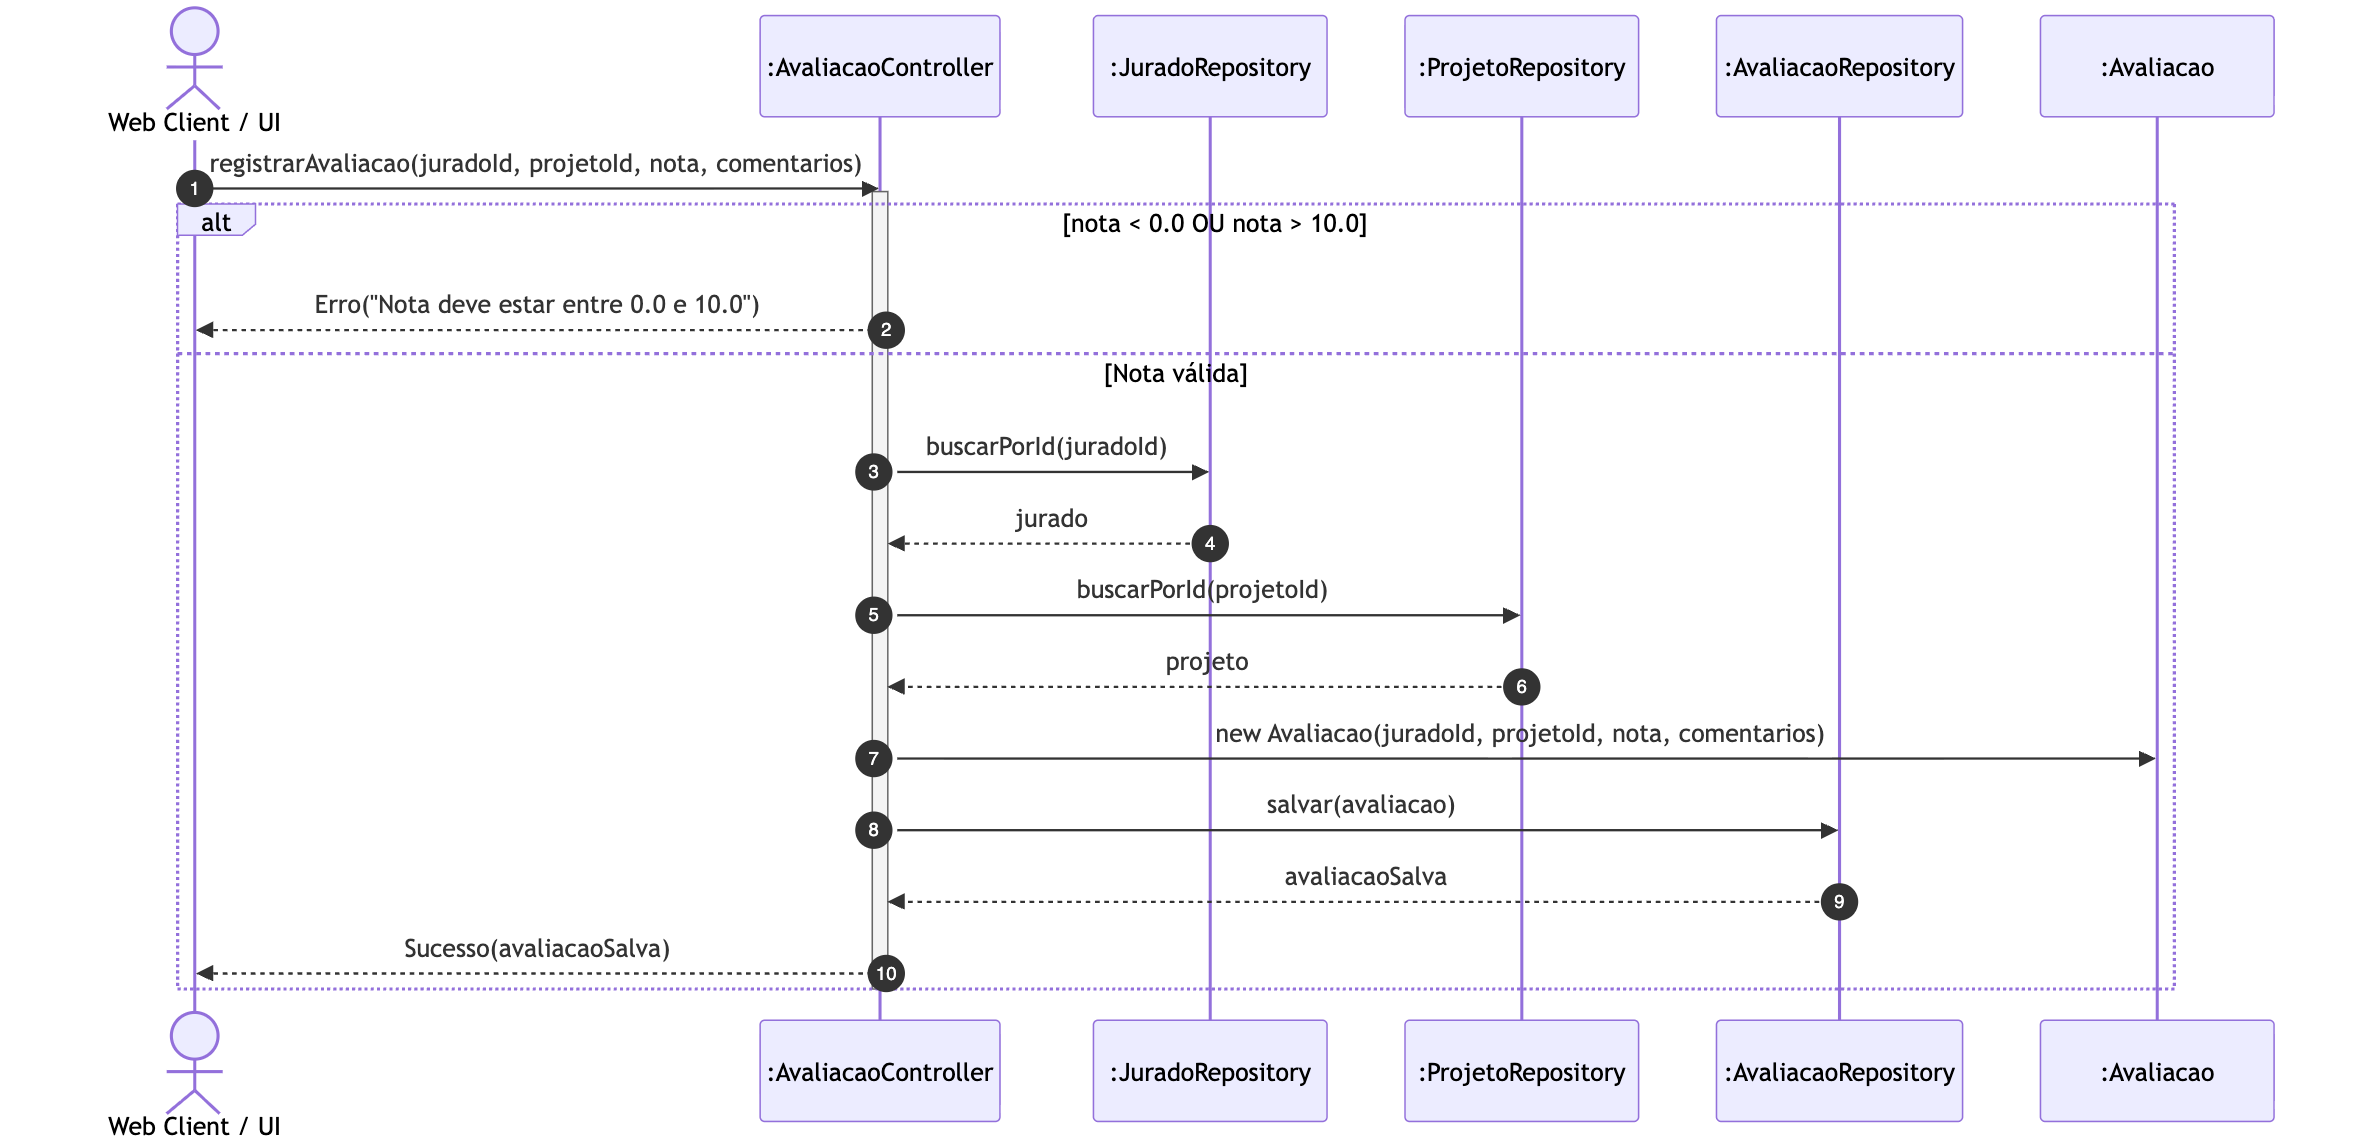
\includegraphics[width=0.92\textwidth]{images/sd_registrar_avaliacao.png}
\caption{Diagrama de Sequência de Projeto: Registrar Avaliação}
\label{fig:sd_registrar_avaliacao}
\end{figure}

\begin{figure}[H]
\centering
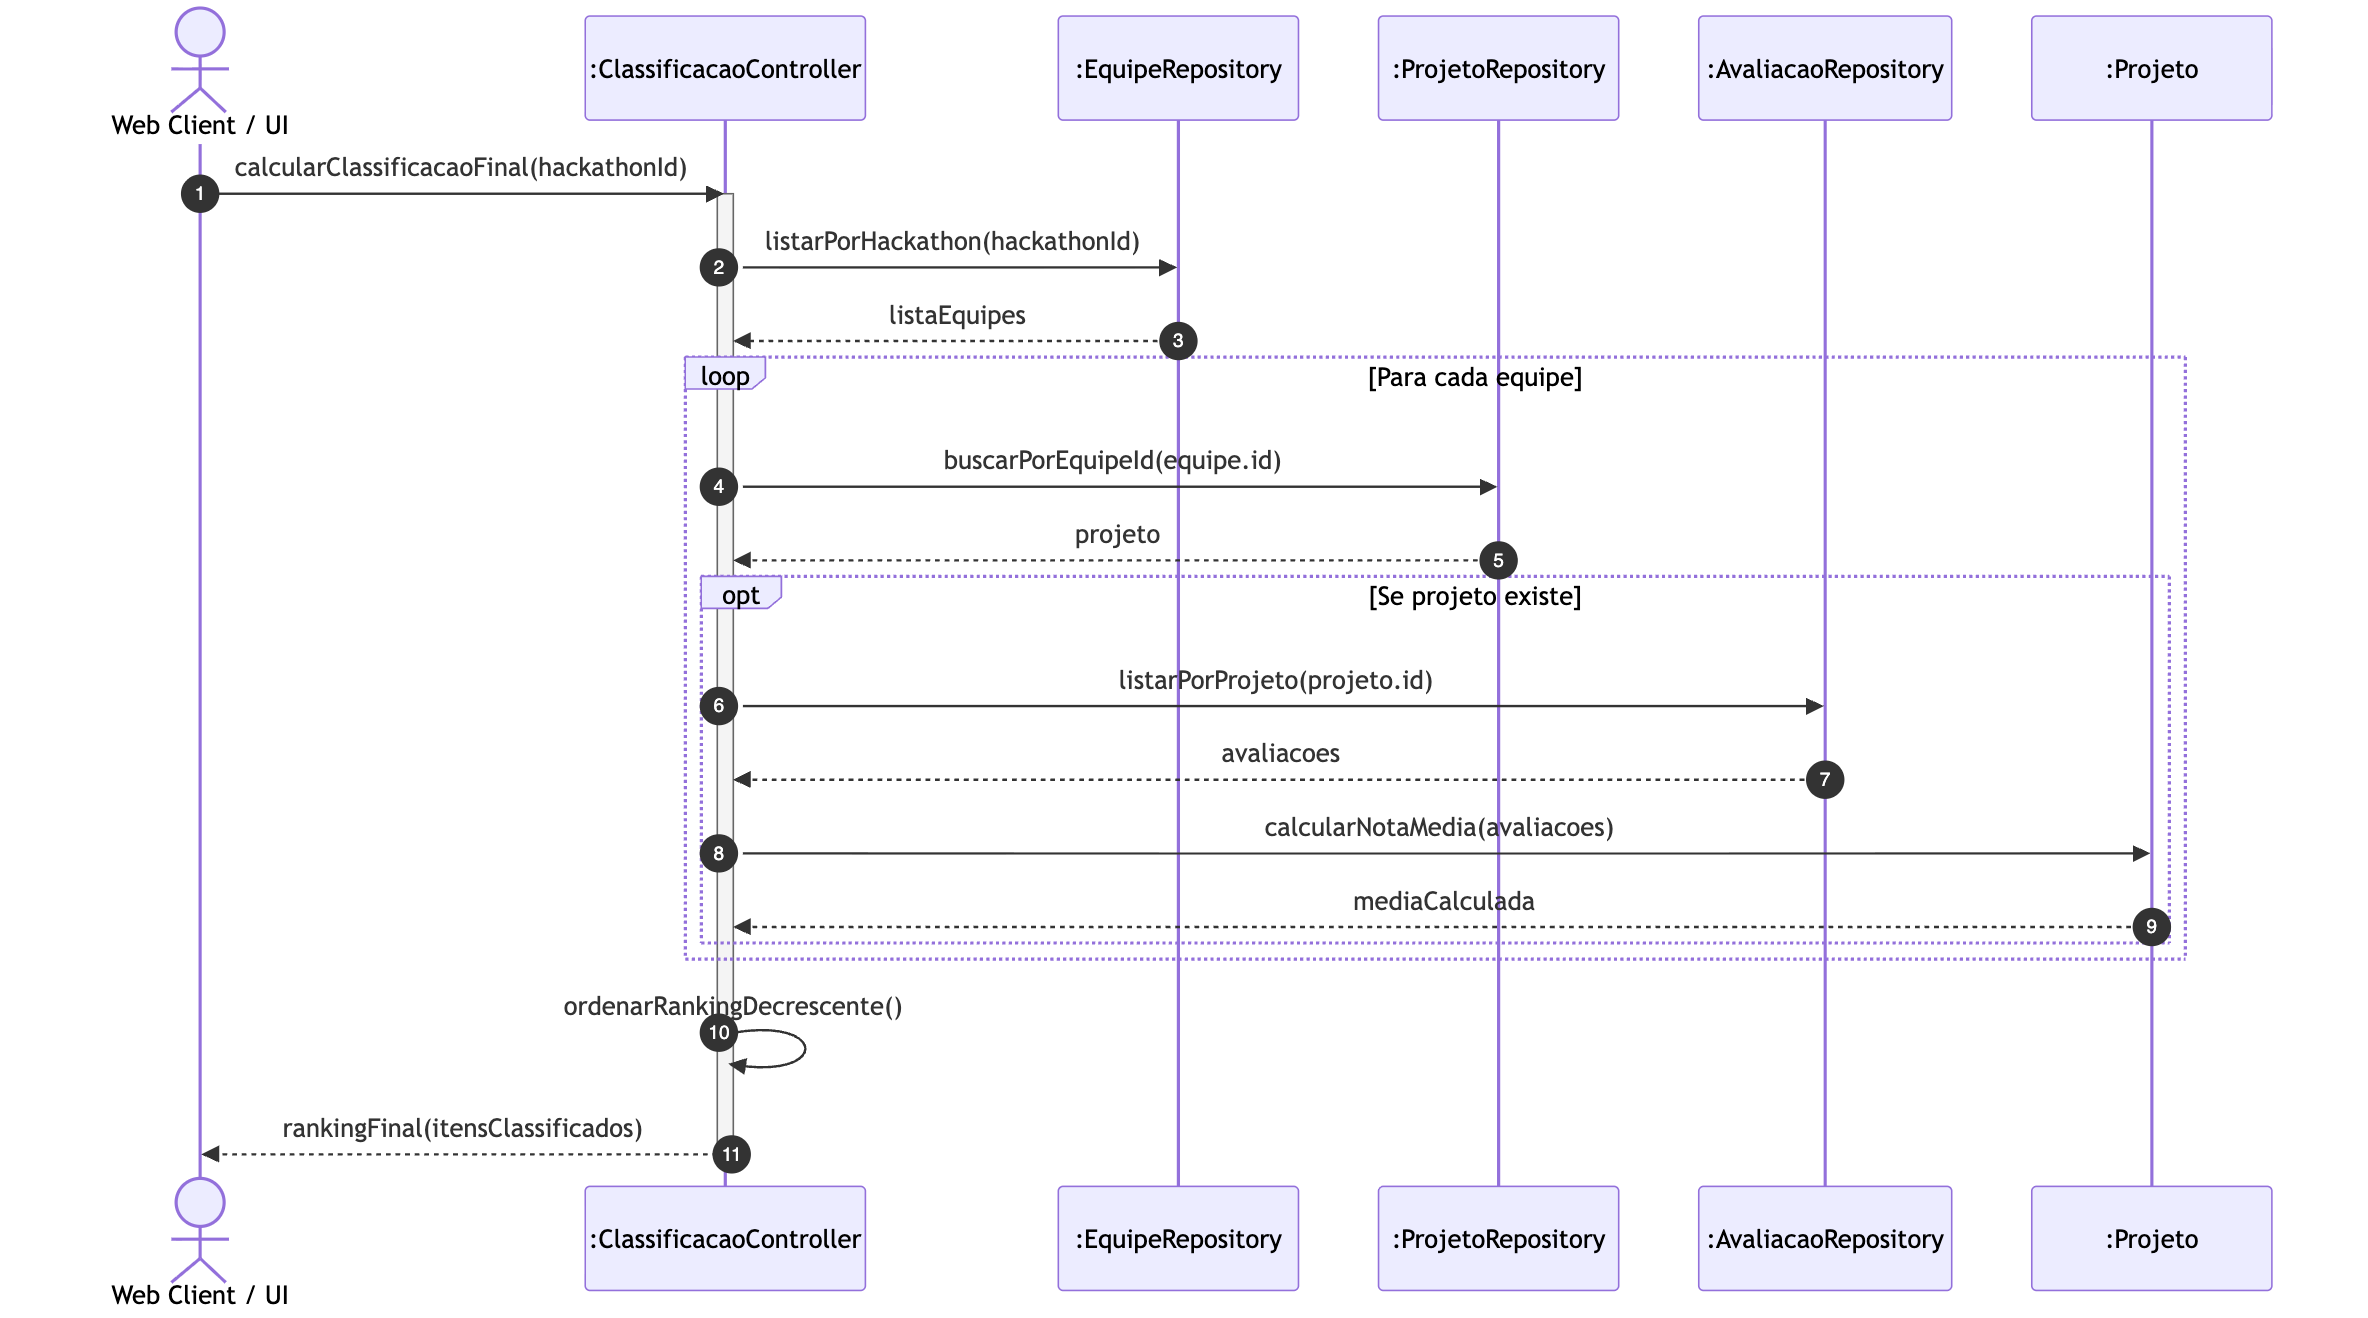
\includegraphics[width=0.92\textwidth]{images/sd_calcular_ranking.png}
\caption{Diagrama de Sequência de Projeto: Determinar Classificação Final}
\label{fig:sd_calcular_ranking}
\end{figure}

\section{Diagrama de Classes de Projeto (DCD) e Pacotes}

O Diagrama de Classes de Projeto (DCD), apresentado na Figura~\ref{fig:dcd}, detalha a estrutura formal das classes do software com visibilidade (+ público, - privado), atributos, métodos e tipos de retorno.

\begin{figure}[H]
\centering
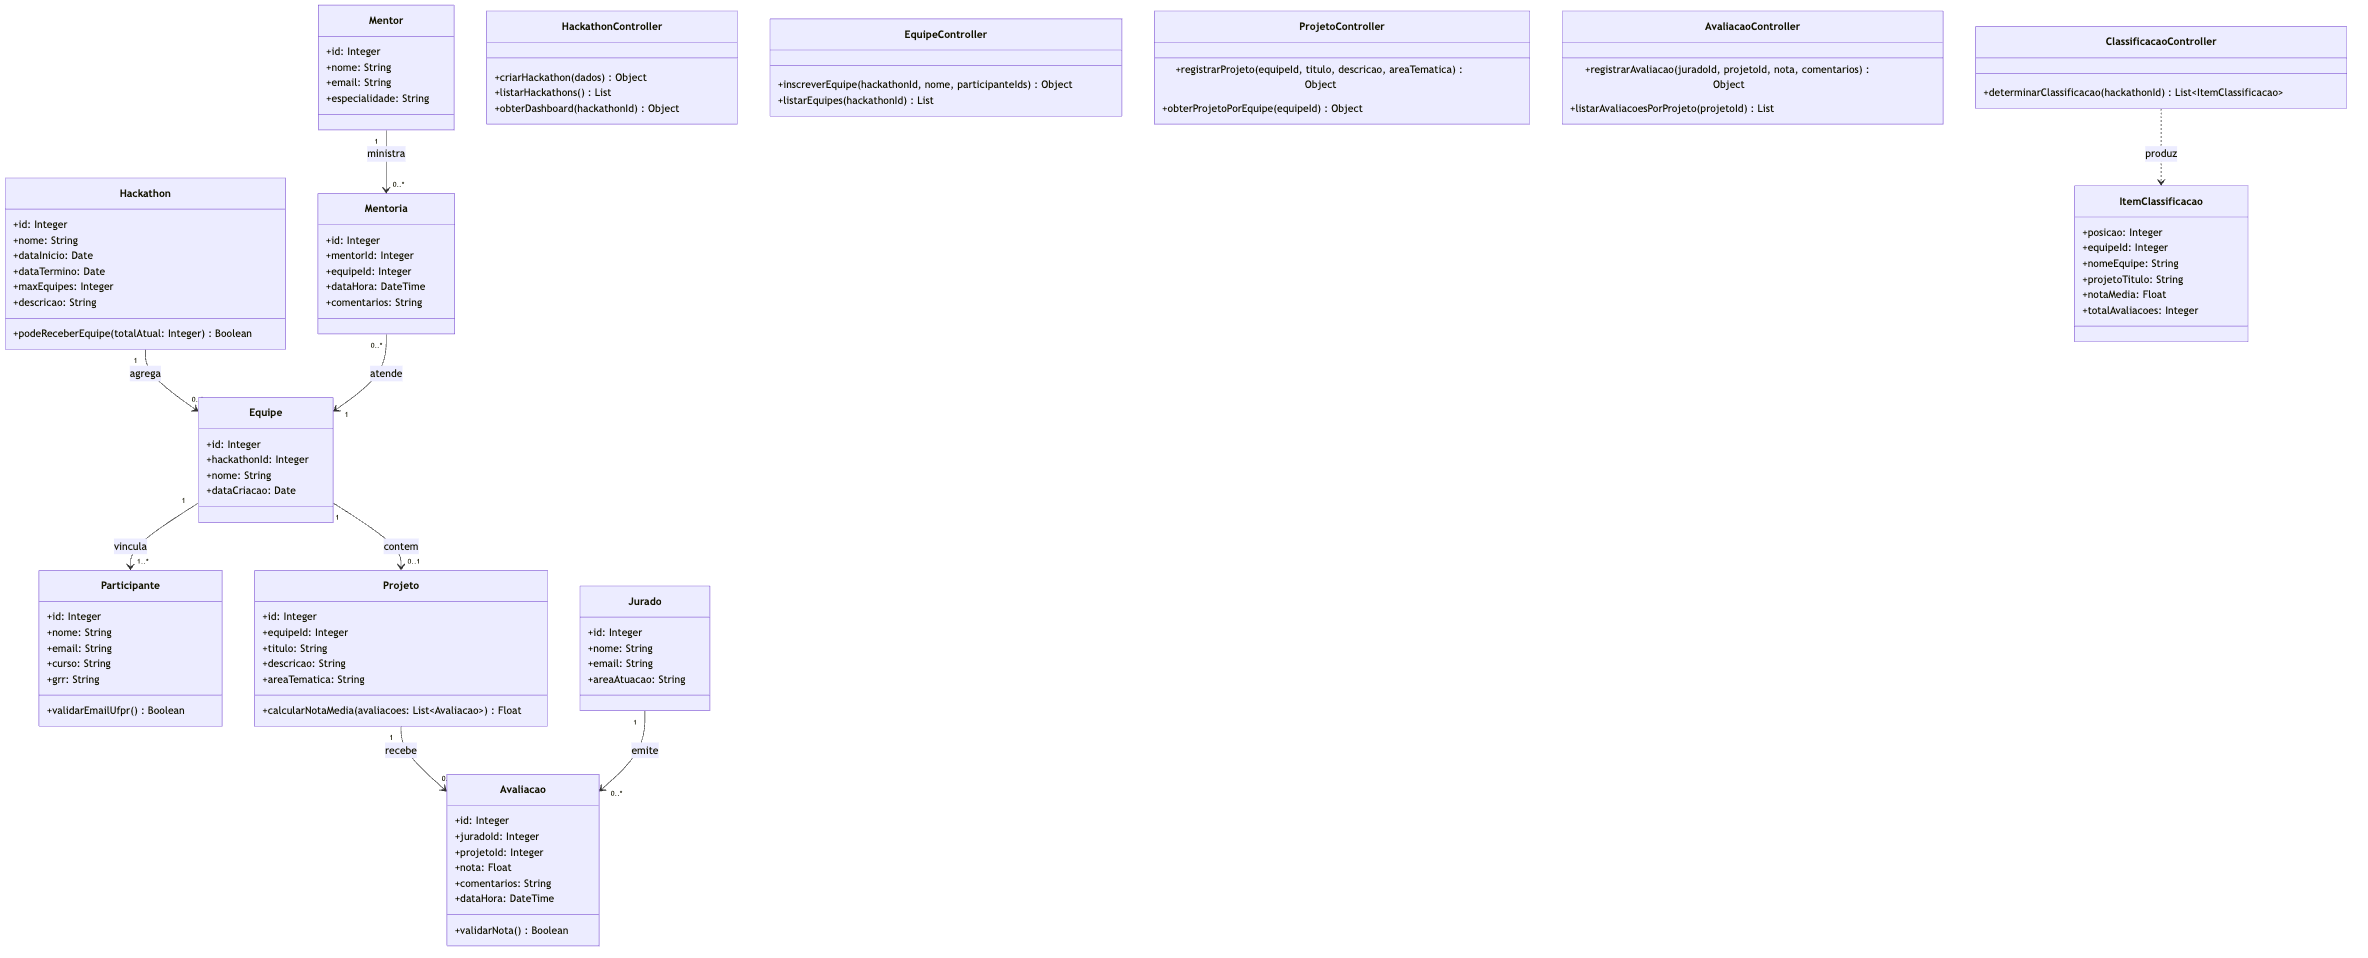
\includegraphics[width=0.98\textwidth]{images/dcd.png}
\caption{Diagrama de Classes de Projeto (DCD)}
\label{fig:dcd}
\end{figure}

A organização modular do software segue o Diagrama de Pacotes apresentado na Figura~\ref{fig:package_diagram}, dividindo o sistema em quatro camadas bem delimitadas:
\begin{itemize}
    \item \textbf{presentation}: SPA React com Tailwind CSS em \texttt{src/client} e rotas REST Fastify em \texttt{src/server/routes}.
    \item \textbf{application}: Controladores GRASP contendo a lógica de orquestração dos casos de uso.
    \item \textbf{domain}: Entidades de negócio e regras de validação de domínio com Zod.
    \item \textbf{infrastructure / repositories}: Repositórios Knex.js com persistência em banco de dados SQLite (\texttt{hackathon.sqlite}).
\end{itemize}

\begin{figure}[H]
\centering
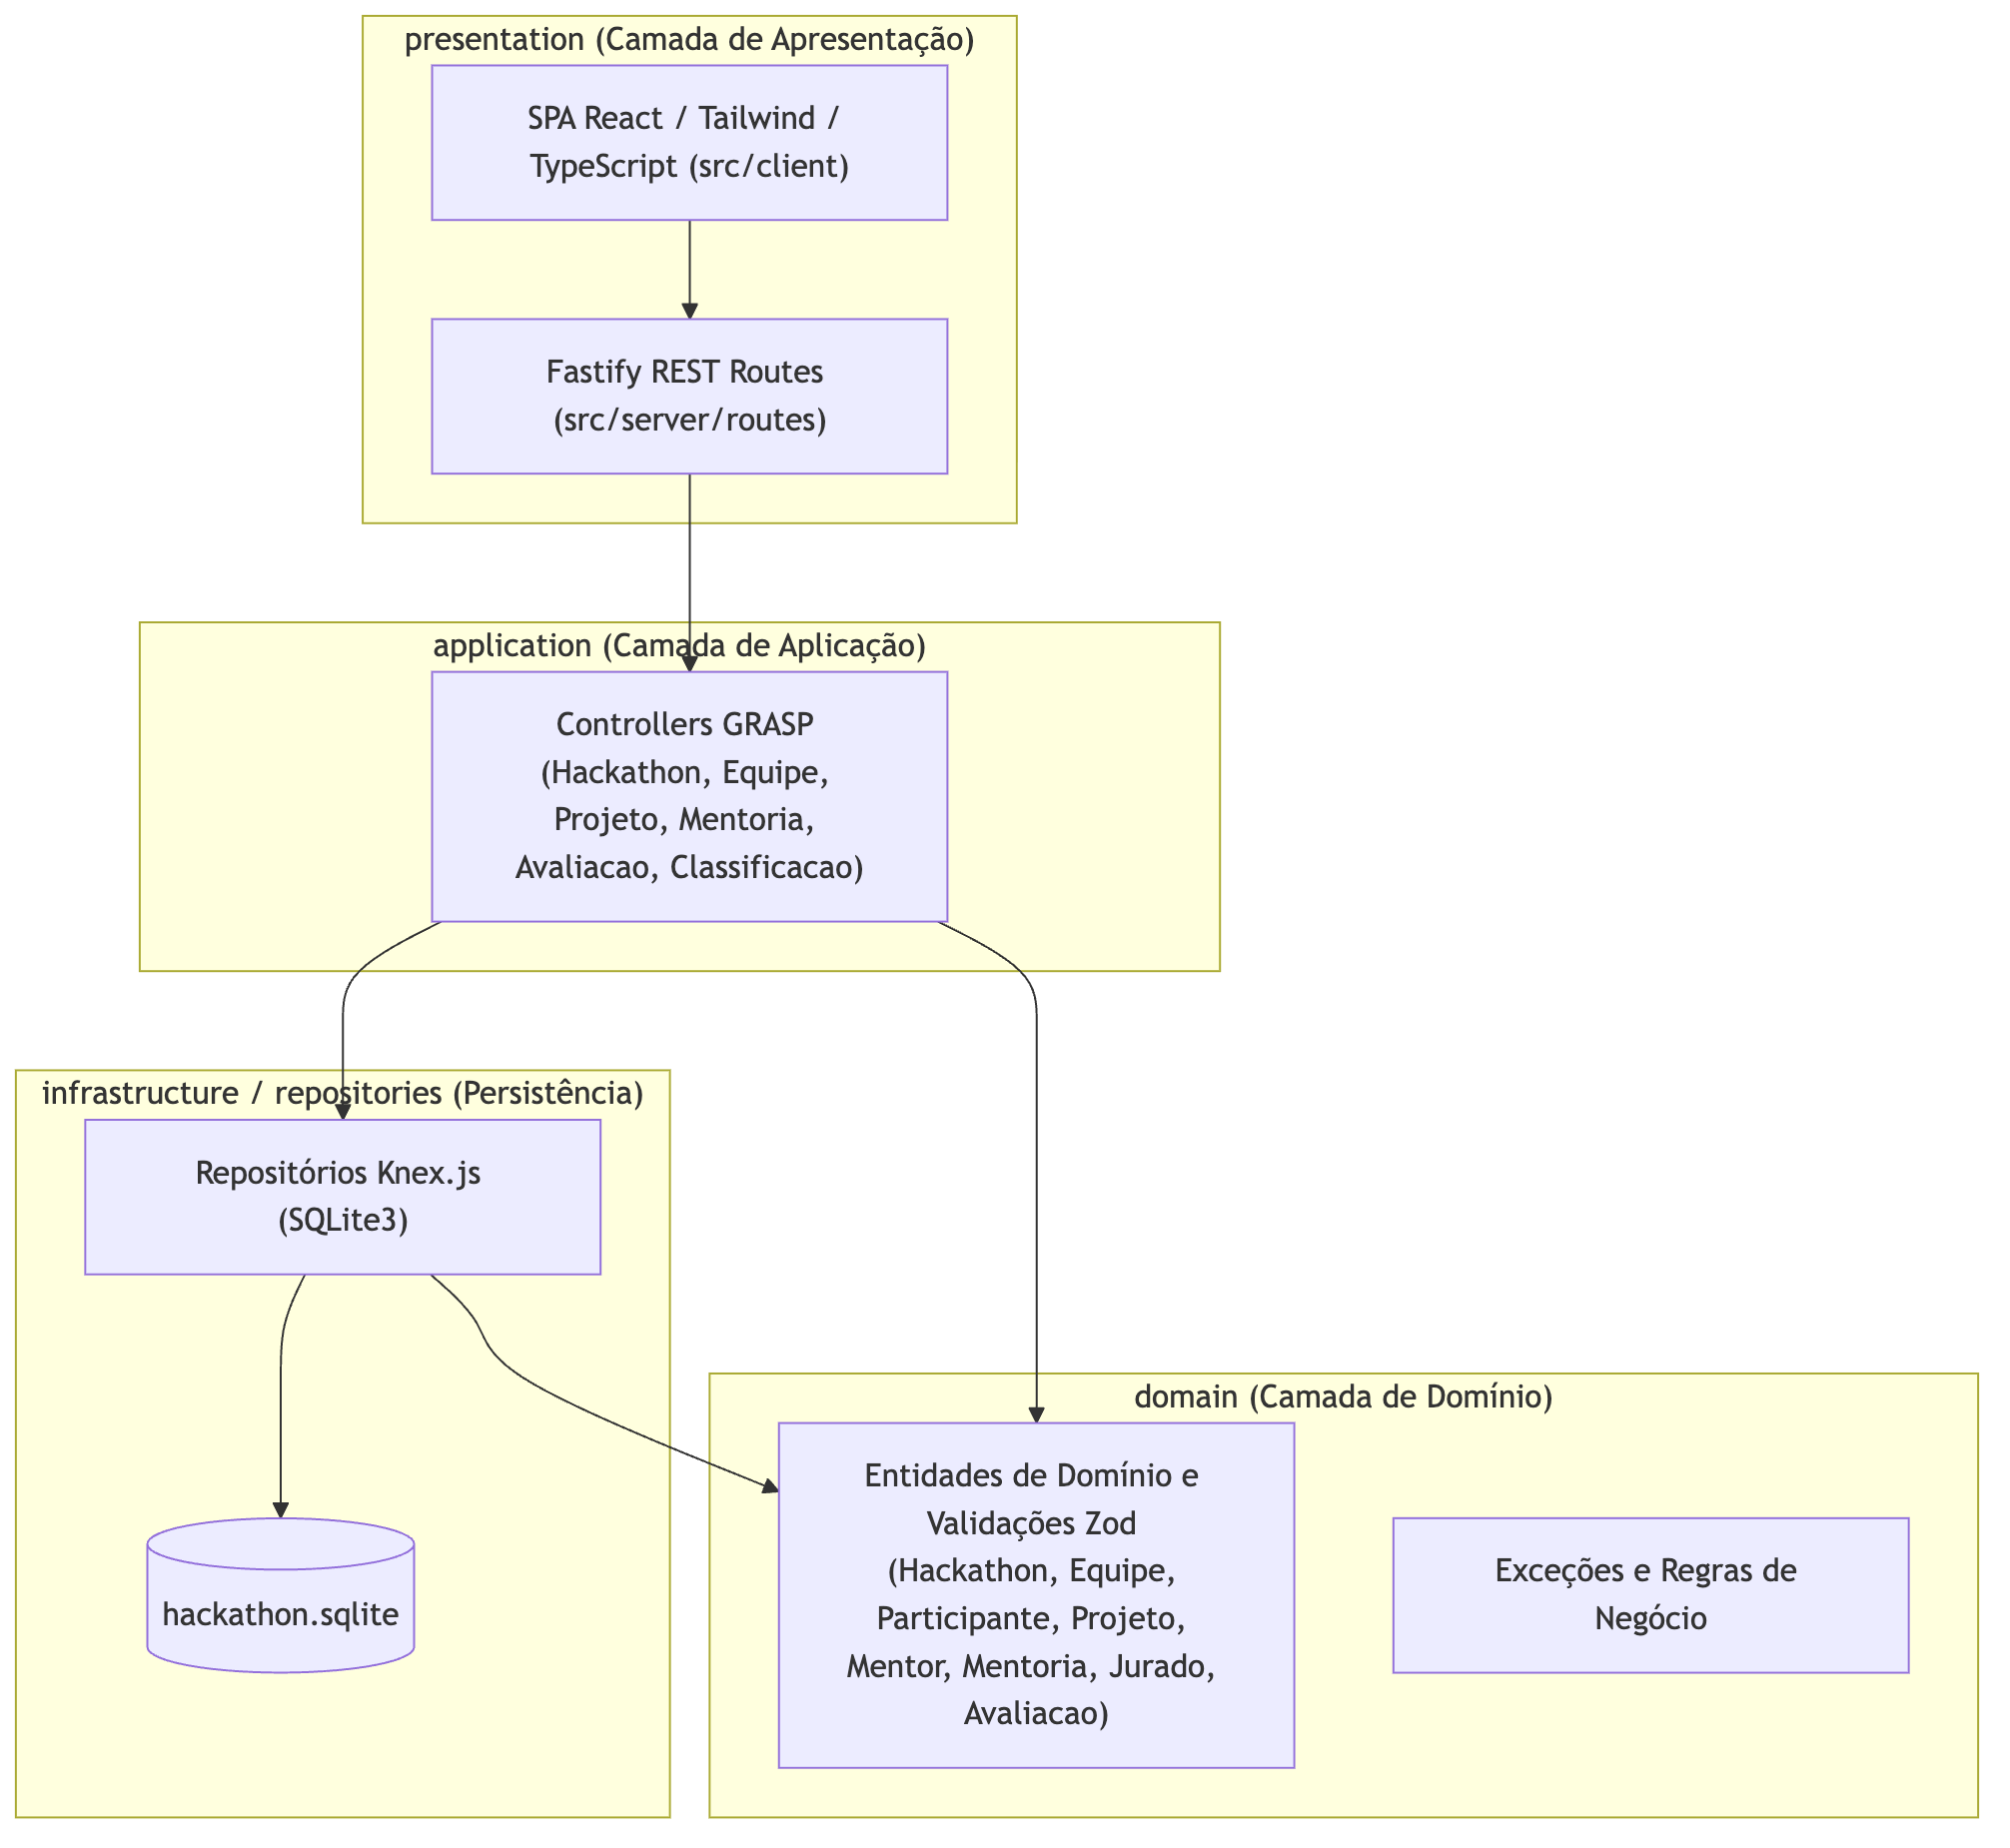
\includegraphics[width=0.9\textwidth]{images/package_diagram.png}
\caption{Diagrama de Pacotes / Arquitetura do Sistema}
\label{fig:package_diagram}
\end{figure}

\section{Estrutura da Implementação e Guia de Execução}

O software foi desenvolvido de forma simples, elegante e totalmente funcional utilizando a seguinte stack tecnológica:
\begin{itemize}
    \item \textbf{Backend}: Node.js com Fastify e Knex.js conectado a banco de dados relacional SQLite3 com tipagem TypeScript e validações Zod.
    \item \textbf{Frontend}: React.js com Vite, TypeScript, Zod e Tailwind CSS localizado em \texttt{src/client}, com navegação organizada por papéis de atores UML:
    \begin{itemize}
        \item \texttt{/organizador}: Criação de hackathons, visão geral e botão de carga instantânea de dados de demonstração da UFPR;
        \item \texttt{/estudante}: Cadastro de participante, inscrição de equipe e registro de projeto;
        \item \texttt{/mentor}: Cadastro de mentor e registro de orientações de mentoria;
        \item \texttt{/jurado}: Cadastro de jurados e lançamento de notas (0 a 10) e pareceres;
        \item \texttt{/ranking} ou \texttt{/}: Pódio e tabela de classificação final em tempo real.
    \end{itemize}
\end{itemize}

\subsection{Como Executar o Sistema}

Para executar a aplicação completa em ambiente local:

\begin{lstlisting}[language=bash]
# 1. Instalar as dependencias e compilar
npm install
cd src/client && npm install && npm run build && cd ../..

# 2. Iniciar o servidor e a aplicacao web
npm start
\end{lstlisting}

O sistema estará disponível no navegador em \url{http://localhost:3000}. Na interface, basta clicar em \textbf{"Carregar Demonstração UFPR"} para popular o banco SQLite com o hackathon, equipes, projetos, mentorias e notas de jurados, permitindo testar todas as funcionalidades imediatamente.

\section{Conclusão}

O projeto e a implementação desenvolvidos atendem com precisão rigorosa a todos os requisitos do edital do Primeiro Trabalho Prático de Engenharia de Software da UFPR. A transição da especificação de requisitos para a modelagem orientada a objetos (Casos de Uso, Modelo de Domínio, DSS, Contratos e GRASP) resultou em uma arquitetura limpa, extensível e desacoplada, perfeitamente refletida no código-fonte em Node.js/SQLite e na interface web React.

\bibliographystyle{sbc}
\bibliography{sbc-template}

\end{document}
